\chapter{Brownian Motion}\label{sec:BM}
\marginpar{\textcolor{red}{Lecture 19}}

bla bla \footnote{was intelligenteres hinschreiben}
\section[Stochastic processes in continuous time]{Introduction to stochastic processes in continuous time}\label{sec:SP}
	Stochastic processes in discrete time have been studied in Chapter \ref{chapter:MT} mostly from the point of view of sequences of random variables. In continuous time things escalate quickly if the index set is uncountable. In this section we lay the foundations of stochastic processes seen as path-valued random variables. This interpretation forces us to discuss quite a bit of measure theory. We will lay the foundations to study the Brownian motion and convergence of sequences of stochastic processes in the general frame-work of weak convergence in Polish spaces from the previous chapter. \smallskip

	Let us first recall the definition of a stochastic process. For a fixed probability space $(\Omega, A, \P)$ a collection $X=(X_t)_{t\in I}$ of random variables with values in a measurable space $(E,\mathcal E)$ is called a stochastic process with state-space $E$. Most of the time we can assume that $E$ is a Polish metric space with Borel $\sigma$-algebra $\mathcal E=\mathcal B(E)$ but always keep in mind the most important example $E=\R$. The index set $I$ was assumed to be discrete in the discussion of martingales but can also be continuous here. The (random) mapping $t\mapsto X_t(\omega)$ is called a trajectory (or sample path) of $X$. While the study of discrete time stochastic processes was rather elementary (playing with stopping times and the martingale property) the study of continuous time processes will be more involved caused by the measure theory on path-space where the continuum appears twice (in space and time). An illustrative task is to answer (or properly define) the question if sample paths of stochastic processes are almost surely continuous or differentiable.\smallskip
	
In order to develop the full theory of stochastic processes we will first extend the triology of measure theory behind random vectors, i.e. stochastic processes with $|I|<\infty$, from Section \ref{sec:RV}:
\begin{itemize}
	\item define a $\sigma$-algebra $\mathcal E^{\otimes I}$ on the generic path space $E^I$,
	\item understand all probability measures on $\mathcal E^{\otimes I}$
	\item reinterprete stochastic processes as path-valued random variables.
\end{itemize}
There is already quite a bit of pain involved in generalizations from finite $I$ to uncountable $I$ and even worse if trajectories are supposed to be continuous, which we study next.

\subsection{Stochastic processes and the generic path space}
The biggest hurdle towards a thorough understanding of continuous-time stochastic processes is the measure theory on path space. Even though the main interest of this course is processes with continuous sample paths (such as the Brownian motion) it is useful to first discuss measure theory on generic functions $f:I\to E$ with absolutely no assumptions on $f$. In the previous chapter we enlarged $[0,\infty)$ to the one-point compactification $[0,\infty]$ in order to gain compactness. It is much less simple to see what is gained if continuous functions $C([0,\infty))$ are enlarged to all generic functions $\R^{[0,\infty)}$. There is only one very non-trivial reason, the Kolmogorov extension theorem that we prove below. Kolmogorov's extension theorem is a theorem that allows to construct measures on the natural $\sigma$-algebra on paths $\R^{\otimes [0,\infty)}$ which combined with the Kolmogorov-Chentsov theorem gives a possibility to construct measures on $C([0,\infty))$ and continuous-times stochastic processes. In order to pass that hurdle we carefully discuss all appearing objects and new ideas, and then pass on to the Brownian motion as an application of the strategy. \smallskip




Before getting started it is useful to visualize and reinterpret the generic path space $\R^I$ of all functions from $I$ to $\R$ for the simplest index sets:
\begin{itemize}
	\item $\R^I$ corresponds to $\R$ if $|I|=1$,
	\item $\R^I$ corresponds to $\R^d$ if $|I|=d$, by reinterpreting a vector as a mapping from $d$ arbitrary time-points (the indices of the vector) to $\R$,
	\item $\R^I$ corresponds to the set of real-valued sequences for $I=\N$,
\end{itemize}

\begin{figure}][h]
	\begin{center}
	\begin{tikzpicture}[scale=0.6,transform shape]
			\tikzset{
			  pics/tick/.style args={#1}{code={
				\draw[line width=0.3mm,inner sep=0mm] (0,-#1) -- (0,#1) ;
				},
			  }
			}
			  \tikzset{
				cross/.pic ={
				  \draw[pic actions,rotate=#1,line width=0.3mm]
					(-3.5pt,0) -- (3.5pt,0)
					(0,-3.5pt) -- (0,3.5pt);
				},
			  }
			\draw[black!90,line width=0.4mm] (0,-1) -- ++(90:3cm);
			%AXIS X
			\draw[black!90,line width=0.4mm] (0,0) --++(0:3.5cm); 
			\draw (1,0) pic[rotate=0] {tick={1mm}} node[yshift=-2.5mm,xshift=2mm,scale=1.2] {$t_1$} ;
			\draw[darkgreen] (1,-0.5) pic {cross={45}} ;
			\draw[orange] (1,0.5) pic {cross={45}} ;
			\draw[red] (1,1.5) pic {cross={45}} ;
		\end{tikzpicture}
		\hspace{3mm}
		\begin{tikzpicture}[scale=0.6,transform shape]
			\tikzset{
			  pics/tick/.style args={#1}{code={
				\draw[line width=0.3mm,inner sep=0mm] (0,-#1) -- (0,#1) ;
				},
			  }
			}
			  \tikzset{
				cross/.pic ={
				  \draw[pic actions,rotate=#1,line width=0.3mm]
					(-3.5pt,0) -- (3.5pt,0)
					(0,-3.5pt) -- (0,3.5pt);
				},
			  }
			\draw[black!90,line width=0.4mm] (0,-1) -- ++(90:3cm);
			%AXIS X
			\draw[black!90,line width=0.4mm] (0,0) --++(0:5.5cm); 
			\draw (1,0) pic[rotate=0] {tick={1mm}} node[yshift=-2.5mm,xshift=2mm,scale=1.2] {$t_1$} ;
			\draw (2,0) pic[rotate=0] {tick={1mm}} node[yshift=-2.5mm,xshift=2mm,scale=1.2] {$t_2$} ;
			\draw (3,0) pic[rotate=0] {tick={1mm}} node[yshift=-2.5mm,xshift=2mm,scale=1.2] {$t_3$} ;
			%t1
			\draw[darkgreen] (1,-0.5) pic {cross={45}} ;
			\draw[orange] (1,0.5) pic {cross={45}} ;
			\draw[red] (1,1.5) pic {cross={45}} ;
			%t2
			\draw[darkgreen] (2,0.5) pic {cross={45}} ;
			\draw[orange] (2,1) pic {cross={45}} ;
			\draw[red] (2,1.5) pic {cross={45}} ;
			%t1
			\draw[darkgreen] (3,1) pic {cross={45}} ;
			\draw[orange] (3,1.5) pic {cross={45}} ;
			\draw[red] (3,2) pic {cross={45}} ;
		\end{tikzpicture}
		\hspace{3mm}
		\begin{tikzpicture}[scale=0.6,transform shape]
			\tikzset{
			  pics/tick/.style args={#1}{code={
				\draw[line width=0.3mm,inner sep=0mm] (0,-#1) -- (0,#1) ;
				},
			  }
			}
			  \tikzset{
				cross/.pic ={
				  \draw[pic actions,rotate=#1,line width=0.3mm]
					(-3.5pt,0) -- (3.5pt,0)
					(0,-3.5pt) -- (0,3.5pt);
				},
			  }
			\draw[black!90,line width=0.4mm] (0,-1) -- ++(90:3cm);
			%AXIS X
			\draw[black!90,line width=0.4mm] (0,0) --++(0:4.5cm); 
			\draw (1,0) pic[rotate=0] {tick={1mm}} node[yshift=-2.5mm,xshift=2mm,scale=1.2] {1} ;
			\draw (2,0) pic[rotate=0] {tick={1mm}} node[yshift=-2.5mm,xshift=2mm,scale=1.2] {2} ;
			\draw (3,0) pic[rotate=0] {tick={1mm}} node[yshift=-2.5mm,xshift=2mm,scale=1.2] {3} ;
			\draw (4,0) pic[rotate=0] {tick={1mm}} node[yshift=-2.5mm,xshift=2mm,scale=1.2] {4} ;
			%\draw (5,0) pic[rotate=0] {tick={1mm}} node[yshift=-2.5mm,xshift=2mm,scale=1.2] {5} ;
			%1
			\draw[darkgreen] (1,0.5) pic {cross={45}} ;
			\draw[orange] (1,1.5) pic {cross={45}} ;
			\draw[red] (1,1) pic {cross={45}} ;
			%2
			\draw[darkgreen] (2,-0.5) pic {cross={45}} ;
			\draw[orange] (2,1.5) pic {cross={45}} ;
			\draw[red] (2,1) pic {cross={45}} ;
			%3
			\draw[darkgreen] (3,0.25) pic {cross={45}} ;
			\draw[orange] (3,0.75) pic {cross={45}} ;
			\draw[red] (3,1.25) pic {cross={45}} ;
			%4
			\draw[darkgreen] (4,0.5) pic {cross={45}} ;
			\draw[orange] (4,1) pic {cross={45}} ;
			\draw[red] (4,1.5) pic {cross={45}} ;
			%5
			%\draw[darkgreen] (5,0.5) pic {cross={45}} ;
			%\draw[orange] (5,1) pic {cross={45}} ;
			%\draw[red] (5,1.5) pic {cross={45}} ;
		\end{tikzpicture}
		\caption*{A few elements of $\R^{\{t_1\}}$, $\R^{\{t_1,t_2,t_3\}}$, and $\R^{\N}$.}
	\end{center}
\end{figure}
	
	




Hence, it is little surprising that we will always try to generalize ideas from $\R^d$ to $\R^I$. Before starting the measure theory on path space the reader might want to have a quick look at the beginning of Section \ref{sec:RV} to recall the steps $\sigma$-algebra, measures, random variables for $\R^d$ as the next sections are similar but much harder in terms of notation.

\subsubsection{(A) The path $\sigma$-algebra}
Recall from Section \ref{sec:Fubini} the notion of a product $\sigma$-algebra. If $\mathcal E$ is a $\sigma$-algebra, then the $d$-fold product $\sigma$-algebra on $E^d$ is defined as 
\begin{align*}
	\mathcal E^{\otimes d}:=\mathcal E\otimes \cdots \otimes \mathcal E:=\sigma(\{B_1\times \cdots \times B_d: B_i\in \mathcal E\}).
\end{align*}
In the sequel the appearing sets $B_1\times \cdots \times B_d$ are called \textbf{boxes} and interpreted using the reinterpretation of $E^d$ as mappings from $d$ arbitrary time-points to $E$.
\begin{figure}[h]
	\begin{center}
    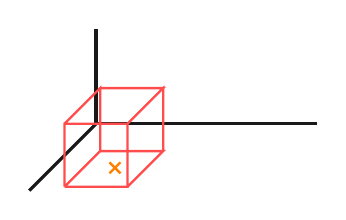
\begin{tikzpicture}[scale=0.8,transform shape]
	\tikzset{
	  pics/tick/.style args={#1}{code={
		\draw[line width=0.3mm,inner sep=0mm] (0,-#1) -- (0,#1) ;
		},
	  }
	}

          \tikzset{
            cube/.pic ={
              \draw[pic actions,line width=0.3mm]
         (0,0) -- ++(0:1cm) -- ++(45:0.8cm) -- ++(0:-1cm) -- ++(45:-0.8cm)
        (0,0) -- ++(0:1cm) -- ++(45:0.8cm) -- ++(0:-1cm) -- ++(45:-0.8cm)
        (0,0) -- ++(90:1cm) --++(45:0.8cm) -- ++(90:-1cm)
        (0,0) -- ++(0:1cm) -- ++(90:1cm) -- ++(45:0.8cm) -- ++(90:-1cm)
        (0,0) -- ++(90:1cm) --++(0:1cm) -- ++(45:0.8cm) --++(0:-1cm);
            }
          }
        \tikzset{
            cross/.pic ={
              \draw[pic actions,rotate=#1,line width=0.3mm]
                (-3.5pt,0) -- (3.5pt,0)
                (0,-3.5pt) -- (0,3.5pt);
            },
          }


        %AXIS Y
        \draw[black!90,line width=0.4mm] (0,0) -- ++(90:1.5cm);
        %AXIS X
        \draw[black!90,line width=0.4mm] (0,0) --++(0:3.5cm);  
        %AXIS Z 
        \draw[black!90,line width=0.4mm] (0,0) --++(45:-1.5cm);  

        %cube 
        \draw[red!70] (-0.5,-1) pic {cube} ;
        \draw[orange] (0.3,-0.7) pic {cross={45}};
     %   \draw[darkgreen] (0.2,0.2) pic {cross={45}}; 
    \end{tikzpicture} 
    \hspace{5mm}
    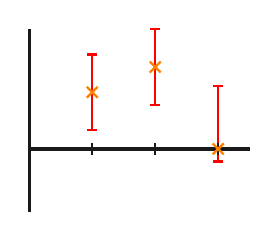
\begin{tikzpicture}[scale=0.8,transform shape]
        \tikzset{
          pics/tick/.style args={#1}{code={
            \draw[line width=0.3mm,inner sep=0mm] (0,-#1) -- (0,#1) ;
            },
          }
        }
        \tikzset{
            cross/.pic ={
              \draw[pic actions,rotate=#1,line width=0.3mm]
                (-3.5pt,0) -- (3.5pt,0)
                (0,-3.5pt) -- (0,3.5pt);
            },
          }
		  \tikzset{
pics/intervall/.style args={#1}{code={
\draw[red,line width=0.3mm] (0,0) -- ++(0,#1) 
node[rotate=90,sloped,inner xsep=0.8mm,inner ysep=0,pos=1,fill,red] (E) {}
node[rotate=90,sloped,inner xsep=0.8mm,inner ysep=0,pos=0,fill,red] (E) {};
},
}
}
\draw  (1,0.3)  pic {intervall={1.2}} ;
\draw  (2,0.7)  pic {intervall={1.2}};
\draw  (3,-0.2)  pic {intervall={1.2}} ;
		  
        %AXIS Y
        \draw[black!90,line width=0.4mm] (0,-1) -- ++(90:2.9cm);
        %AXIS X
        \draw[black!90,line width=0.4mm] (0,0) --++(0:3.5cm);  
        \draw[black!90] (1,0) pic {tick={1mm}};
        \draw[black!90] (2,0) pic {tick={1mm}};
        \draw[black!90] (3,0) pic {tick={1mm}};
       
      %  \draw[darkgreen] (1,1) pic {cross={45}};
        \draw[orange] (1,0.9) pic {cross={45}};
        %\draw[red,line width=0.3mm] (1,0.3) -- ++(90:12mm);

        %\draw[red,line width=0.3mm] (2,0.7) -- ++(90:12mm);
        %\draw[darkgreen] (2,0.8) pic {cross={45}};
        \draw[orange] (2,1.3) pic {cross={45}};

        %\draw[red,line width=0.3mm] (3,0) -- ++(90:12mm);
        %\draw[darkgreen] (3,1) pic {cross={45}};
        \draw[orange] (3,0) pic {cross={45}};
    \end{tikzpicture}
	\caption*{Reinterpretation of a three-dimensional box for arbitrary three time-pointes}
\end{center}
\end{figure}


If $\mathcal E=\sigma(\mathcal A)$, then $\mathcal E^{\otimes d}$ can also be expressed as
\begin{align*}
	\mathcal E^{\otimes d}=\sigma(\{B_1\times \cdots \times B_d: B_i\in \mathcal A\}).
\end{align*}
Most importantly, if $E=\R$ and $\mathcal A$ is chosen as the set of intervals than the product $\sigma$-algebra is generated by rectangular sets. The aim is to introduce a generalization to infinite products, but what is a good notion for a (possibly uncountable) infinite product of sets?
As usually in Mathematics the trick is to reduce as far as possible to the finite case:
\begin{ldef}
	\begin{deff}
		A subset $C$ of $E^I$ is called \textbf{finitely generated cylinder set} if 
		\begin{align*}
			C&=\pi_{J}^{-1}(B_1\times \cdots \times B_n)\\
			&=\{f:I\to E\,|\, f(t_1)\in B_1, ..., f(t_n)\in B_n\},
		\end{align*}
		where $J=\{t_1,...,t_n\}\subseteq I$ and $B_1,...,B_n\in \mathcal E$. The projections $$\pi_{J}(f)=(f(t_1),...,f(t_n))$$ evaluate a path at finitely many given time-points. We say $C$ is spanned by the time-points $t_1,...,t_d$ and the box $B_1\times \cdots \times B_d \in \mathcal E^{\otimes n}$.	
		%To abbreviate we also write $C_J^B$ for the finite subset $J=\{t_1,...,t_n\}$ of $I$ and $B=B_1\times \cdots B_n$.
	\end{deff}
\end{ldef}
Before proceeding it is extremely important to gain a visual understanding of  finitely generated cylinder sets. The picture to keep in mind is that of a box tied to the time-points with all possible functions $I\to E$ passing through the box. The set we are speaking about is not the box but that of all such functions!


\begin{figure}[h]
\begin{center}
	\begin{tikzpicture}
	\tikzset{
	  pics/tick/.style args={#1}{code={
		\draw[line width=0.3mm,inner sep=0mm] (0,-#1) -- (0,#1) ;
		},
	  }
	}
\tikzset{
pics/intervall/.style args={#1}{code={
\draw[red,line width=0.3mm] (0,0) -- ++(0,#1) 
node[rotate=90,sloped,inner xsep=0.8mm,inner ysep=0,pos=1,fill,red] (E) {}
node[rotate=90,sloped,inner xsep=0.8mm,inner ysep=0,pos=0,fill,red] (E) {};
},
}
}
	%AXIS Y
	\draw[black!90,line width=0.4mm] (0,-0.6) -- ++(90:2.5cm);
	%AXIS X
	\draw[black!90,line width=0.4mm] (0,0) --++(0:3.5cm);  
	\draw (1,0) pic[rotate=0] {tick={1mm}} node[yshift=-2.5mm,xshift=2mm,scale=1.2] {$t_1$} ;
	\draw (2,0) pic[rotate=0] {tick={1mm}} node[yshift=-2.5mm,xshift=2mm,scale=1.2] {$t_2$} ;
	\draw (3,0) pic[rotate=0] {tick={1mm}} node[yshift=-2.5mm,xshift=2mm,scale=1.2] {$t_3$} ;

  \draw  (1,0.5)  pic {intervall={0.6}} ;
  \draw  (2,0.5)  pic {intervall={0.6}};
  \draw  (3,0.1)  pic {intervall={0.6}} ;
	
  %func 1 
  \draw[orange,line width=0.3mm] (0,0.5) .. controls (1.5,1.5) and  (2,0.4) .. (2.5,0.8);
  \draw[orange,line width=0.3mm] (2.5,0.4) .. controls (3,0)  .. (3.5,0.8);

  %func 2
  \draw[blue,line width=0.3mm] (0,1.5) .. controls (1,0.5) .. (1.8,0.8);
  \draw[blue,line width=0.3mm] (1.8,0.9) .. controls (2,0.8)  .. (2.5,1.1);
  \draw[blue,line width=0.3mm] (2.5,1.3) .. controls (3,0.1)  .. (3.5,0.3);

  %func 3
  \draw[darkgreen,line width=0.3mm] (0,1) .. controls (1,0.5) and (2,1.3) .. (3.5,0.2);
\end{tikzpicture} 
\caption*{The cylinder set is the set of all functions passing through the box tied at times from $J$}
\end{center}
\end{figure}

	There are two quantities that have to be distinguished very carefully. The spanning box, which is a finite-dimensional measurable set, and the cylinder set which is a set of functions. 
\begin{ldef}
\begin{deff}
		 The \textbf{path $\sigma$-algebra} (or \textbf{product $\sigma$-algebra}) $\mathcal E^{\otimes I}$ on $E^I$ is the smallest $\sigma$-algebra that contains all finitely generated cylinder sets.
		In the special case $(\R,\mathcal B(\R))$ one typically writes $\mathcal B(\R^d)$, $\mathcal B(\R^\infty)$, $\mathcal B(\R^{[0,T]})$ to abbreviate the notation and also speaks of the product $\sigma$-algebra.
	\end{deff}
\end{ldef}
To get an idea of the definition it is useful to compare the cases $|I|=d$ and $I=\N$ for $E=\R$. For the first the cylinder sets are just boxes. Some of the $B_i$ will typically be equal to $E$, not imposing a restriction. The path $\sigma$-algebra is nothing but the well-known $d$-fold product $\mathcal B(\R^d)=\mathcal B(\R)^{\otimes d}$ from Section \ref{sec:ZV}. This motivates why sometimes we call path $\sigma$-algebras product $\sigma$-algebra also for infinite index sets $I$. The infinite product structure becomes more visible for $I=\N$, where the finitely generated cylinder sets are actually infinite products of the type $\R\times B_1 \times \cdots \times B_2\times \R \times \cdots$ as the factors $\R$ impose no restriction. While the infinite cartesian product makes sense for sequences the good way of writing an uncountable product with restrictions at finitely many time-points is the formalism using projections on finitely many time-points.\smallskip


Here are two simple exercise that we will later need and that is very useful to get acquainted with the new definitions.
\begin{luebung}
	Show that the set of all finitely generated cylinder sets form a semiring. First draw some pictures and then try to formalize your findings using projections.
\end{luebung}



As always there are many different generators of the $\sigma$-algebra, not all are equally useful.
\begin{luebung}
	Suppose that $\mathcal E=\sigma(\mathcal A)$. Check that 
	\begin{align*}
		\mathcal E^{\otimes I}&= \sigma( \{\pi^{-1}_{t_1,...,t_n}(B_1\times \cdots \times B_n):n\in\N, t_i\in J, B_i\in \mathcal A\})\\
		\mathcal E^{\otimes I}&= \sigma( \{\pi_i^{-1}(B):i \in I, B\in  \mathcal E \}),\\	
		\mathcal E^{\otimes I}&= \sigma( \{\pi_i^{-1}(B):i \in I, B\in  \mathcal A\}),
	\end{align*}
	and draw some examples of sets of paths in the generators of $\mathcal E^{\otimes I}$.	Which of the generators of $\mathcal E^{\otimes I}$ is intersection stable?
\end{luebung}
If $|I|<\infty$ or $I$ is countable not much more needs to be said, there are no bad surprises, everything works more or less similarly to $\mathcal B(\R^d)$. The only trouble is the usual difference between $\mathcal P(\R^d)$ and $\mathcal B(\R^d)$ that arises from the fact that countable set operations in a $\sigma$-algebra do not allow to approximate arbitrary subsets from $\R^d$ using intervals/open sets/closed sets/etc. Most interesting sets of interest belong to $\mathcal B(\R^d)$, the generator is rich enough. The story is very different for uncountable index sets $I$ because a second and more severe uncountability issue appears. The generator of $\mathcal E^{\otimes I}$ only uses single (or finitely many) points in time which is by far not enough to capture a lot of information about functions in time. It is instructive to compare with Example \ref{bspd} where it was shown that the smallest $\sigma$-algebra containing singletons can only cover the countable sets. Hence, the finitely generated cylinder sets can at most cover countably generated cylinder with the meaning that a set of functions $C$ is countably generated if there is a countable set of time-points $J\subseteq I$ 
such that  \footnote{alle generatoren durchdenken}
\begin{align*}
	f\in C\quad \Leftrightarrow \quad f_{|J}\in B
\end{align*}
for some $B\in \mathcal E^{\otimes J}$. Equivalently, $C=\pi^{-1}_J(B)$ with the projection $\pi_J$ on infinitely many time-points, the sets of functions with restrictions at countably many time-points.
\begin{llemma}
\begin{prop}
	The set $\mathcal V$ of all \underline{countably} generated cylinder sets is a $\sigma$-algebra on $E^I$ that contains $\mathcal E^{\otimes I}$.%, where a set $A\subseteq E^I$ is called countably generated if there is a countable subset $J\subseteq I$ and a set $B\in \mathcal E^J$ such that 
	%\begin{align*}
	%	f\in A\quad \Leftrightarrow \quad f_{|J}\in B.
	%\end{align*}
\end{prop}
\end{llemma}
\begin{proof}[Proof]
	To check the three properties of a $\sigma$-algebra is straight forward.\smallskip

	(i) Choosing $J$ to be an arbitrary singleton and $B=E$ proves that $\Omega=E^I$ is countably generated.\smallskip
	
	(ii) If $C$ is generated at some countable set of times $J$, then $C^c$ (the path that do not pass through the given sets at some time $t\in J$) can be written as union of the countably many cylinder sets that pass through $B_t^c$ at time $t\in J$.
	
	
	
	then also $C^c$ is countably generated by the same time-points $J$ using $B^c$.\footnote{schnitt!}\smallskip

	(iii) Suppose $C_1,...$ are generated by countable sets $J_1, J_2,...$ and corresponding sets $B_1,B_2,...$. Then also the union $J:=\cup_{k=1}^\infty J_k$ is countable and $\cup_{k=1}^\infty C_k$ is generated by $J$ and\footnote{noch sauber hinschreiben} $B:=B_1\times B_2\times ... \in \mathcal E^{\otimes J}$.\smallskip 

	Since all finitely generated sets are also infinitely generated the generator of $\mathcal E^{\otimes I}$ is a subset of $\mathcal V$. Hence, $\mathcal E^{\otimes I}\subseteq \sigma(\mathcal V)=\mathcal V$ which is the claim.
\end{proof}
The proposition has dramatic consequences! Almost all sets of paths that we might be interested in to study the behavior of paths $t\mapsto X_t(\omega)$ are \textbf{not} measurable in the path $\sigma$-algebra!
\begin{example}
	Suppose $E=\R$ and $I=\R$, $I=[0,1]$, or $I=[0,\infty)$. 
	\begin{itemize}
	\item Singleton sets $\{f\}$ containing only a single path are not measurable.
	\item The set of all constant functions $\{f\equiv c\,|\,c\in E\}$ is not measurable.
	\item The set of non-negative functions $\{ f:I\to E\,|\, f\geq 0\}$ is not measurable.
	\item The set of all continuous functions $\{f:I\to E\,|\, f\text{ continuous}\}$ is not measurable.
	\item  The set of all differentiable functions $\{f:I\to E\,|\, f\text{ differentiable}\}$ is not measurable.
	\end{itemize}
\end{example}
The reason is simple. If any of those sets was measurable in the $\sigma$-algebra $\R^{\otimes I}$ of paths, then there should be a countable set $J$ of time-points that spans the set. If $I$ is uncountable there is an index $i\notin J$. Now take a function $f$ from the sets and add some value at $i$ that destroys the defining property. Then the new function $\tilde f$ is still in the set as the values on $J$ are not changed. But then the set contains a function that violates the defining property which should not be the case. As a consequence we should be very careful with statements of the kind "{}$\P$-almost all paths are continuous"{} with measures on the uncountable product $\sigma$-algebras on paths.\smallskip

Since uncountable product $\sigma$-algebras are delicate one should ask if the decision to work with $\mathcal E^{\otimes I}$ was clever or non-sense. The surprising answer is clever as there is a natural way to construct measures on $\mathcal E^{\otimes I}$ and most delicate issues about zero sets and path properties can be resolved.

\subsubsection{(B) Probability measures on paths}
The aim of this section is to identify all probability measures on the product $\sigma$-algebra $\mathcal E^{\otimes I}$. For $E=\R$ and $|I|<\infty$ this has already been done in Section \ref{sec:VF}, we now generalize to arbitrary $I$ and $E$ as long as $E$ is a Polish space. The strategy is not simple but can be compared to the theory of distribution functions for probability measures on $\mathcal B(\R)$. Recall the approach from Section \ref{sec:VF}:
\begin{enumerate}[label=(\roman*)]
	\item Downsize the information of a measure into something simple that uniquely characterizes the measure. In that case the simplest $\cap$-stable generator of $\mathcal B(\R)$ was the set of all intervals and we defined $F(t)=\P((-\infty,t])$, $t\in\R$.
	\item Identify natural properties of the simpler object. We used continuity of measures to deduce monotonicity, limits at infinity, and right-continuity for $F$. Such functions were then called distribution functions.
	\item Reverse the game: Show that for all distribution function there is a corresponding probability measure (Carath\'eodory extension theorem)
\end{enumerate}
The approach for measures on $\mathcal E^{\otimes I}$ is exactly the same.
\begin{enumerate}[label=(\roman*)]
	\item Downsized $\P$ by only considering events from the finite cylinder sets (which are $\cap$-stable). This leads to so-called finite dimensional distributions $\P_J$ on $\mathcal E^{\otimes J}$ for all finite subsets $J\subseteq I$.
	\item Check that the family $\{\P_J: |J|<\infty\}$ of all finite dimensional distributions satisfies a natural property, consistency.
	\item Reverse the game: Show that for all consistent families of finite dimensional distributions there is a corresponding probability measures (Carath\'eodory consistency theorem).
\end{enumerate}
The only trouble of the approach comes from the notation. The notation with cylinder sets and finite dimensional distributions is either very long (writing out all appearing cylinder sets) or very compact (abbreviating all cylinder sets). We will stick to the compact way but add figures with illustrations.\smallskip

Here is the first step, the restrictions to the $\cap$-stable generator of finitely generated cylinder sets.
\begin{ldef}
\begin{deff}\label{def:SL}
	If $\P$ is a probability measure on $\mathcal E^{\otimes I}$ and $J\subseteq I$ is finite, then the unique measure on $\mathcal E^{\otimes J}$ defined by
	\begin{align*}
		\P_J(B_1\times \cdots \times B_{|J|}):=\P(\pi_{J}^{-1}((B_1\times \cdots \times B_{|J|})),\quad B_i\in \mathcal E,
	\end{align*}
	is called a \textbf{finite dimensional marginal distribution} of $\P$.
\end{deff}
\end{ldef}
Here is a very important point to understand. On the one hand we have boxes (measurable sets of a finite-dimensional space) on the other hand we have cylinder sets of functions passing through the boxes at time-points $J$ (measurable sets of an infinite-dimensional space). The finite dimensional marginals are the measures that we get by crossing out the functions and only keep the marginals at time $J$.

\begin{figure}[h]
	\begin{center}
    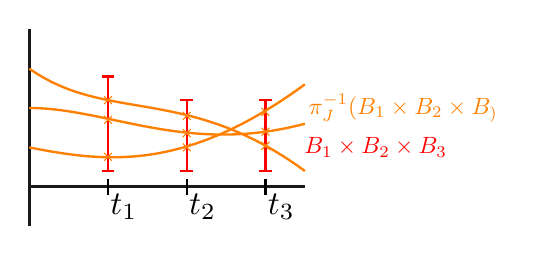
\begin{tikzpicture}
    \tikzset{
      pics/cross/.style args={#1,#2}{code={
      \draw[rotate=#1] (-#2pt,0) -- (#2pt,0)
        (0,-#2pt) -- (0,#2pt);
      },
    }
    }
    \tikzset{
      pics/tick/.style args={#1}{code={
        \draw[line width=0.3mm,inner sep=0mm] (0,-#1) -- (0,#1) ;
        },
      }
    }
\tikzset{
  pics/intervall/.style args={#1}{code={
    \draw[red,line width=0.3mm] (0,0) -- ++(0,#1) 
    node[rotate=90,sloped,inner xsep=0.8mm,inner ysep=0,pos=1,fill,red] (E) {}
    node[rotate=90,sloped,inner xsep=0.8mm,inner ysep=0,pos=0,fill,red] (E) {};
  },
}
}
        %AXIS Y
        \draw[black!90,line width=0.4mm] (0,-0.5) -- ++(90:2.5cm);
        %AXIS X
        \draw[black!90,line width=0.4mm] (0,0) --++(0:3.5cm);   

        \draw (1,0) pic[rotate=0] {tick={1mm}} node[yshift=-2.5mm,xshift=2mm,scale=1.2] {$t_1$} ;
        \draw (2,0) pic[rotate=0] {tick={1mm}} node[yshift=-2.5mm,xshift=2mm,scale=1.2] {$t_2$} ;
        \draw (3,0) pic[rotate=0] {tick={1mm}} node[yshift=-2.5mm,xshift=2mm,scale=1.2] {$t_3$} ;

      \draw  (1,0.2)  pic {intervall={1.2}} ;
      \draw  (2,0.2)  pic {intervall={0.9}};
      \draw  (3,0.2)  pic {intervall={0.9}} ;

      \draw[orange] (1,0.38) pic {cross={45,2}};
      \draw[orange] (1,0.85) pic {cross={45,2}};
      \draw[orange] (1,1.1) pic {cross={45,2}};

      \draw[orange] (2,0.5) pic {cross={45,2}};
      \draw[orange] (2,0.9) pic {cross={45,2}};
      \draw[orange] (2,0.68) pic {cross={45,2}};

      \draw[orange] (3,0.7) pic {cross={45,2}};
      \draw[orange] (3,0.95) pic {cross={45,2}};
      \draw[orange] (3,0.52) pic {cross={45,2}};
        
      \draw[orange,line width=0.3mm] (0,0.5) .. controls (1,0.3) and  (2,0.2) .. (3.5,1.3);
      \draw[orange,line width=0.3mm] (0,1) .. controls (1,1) and  (2,0.4) .. (3.5,0.8);
      \draw[orange,line width=0.3mm] (0,1.5) .. controls (1,0.8) and  (2,1.3) .. (3.5,0.2);

    % \draw[red] (0.5,1) pic {cross={45,8}};
    %\draw[black,line width=0.2mm] (0.2,0.3) -- ++(65:1.2cm);
    %\draw[black,line width=0.2mm] (0.2,1.5) -- ++(-65:1.35cm);
%
 %   \draw[black,line width=0.2mm] (1.3,0.3) -- ++(65:1cm);
  %  \draw[black,line width=0.2mm] (1.3,1.2) -- ++(-65:1cm);
%
 %   \draw[black,line width=0.2mm] (2.3,0.3) -- ++(65:0.8cm);
  %  \draw[black,line width=0.2mm] (2.3,1) -- ++(-65:0.8cm);


    \node[orange,scale=0.85] (pi) at (4.6,1) {$\quad\pi_{J}^{-1}(B_1\times B_2\times B_)$} ;
    \node[red,scale=0.85] (B) at (4.25,0.5) {$\quad B_1\times B_2\times B_3$} ;
    \end{tikzpicture} 
  \caption*{restricting the functions at J = $\{t_1,t_2,t_3\}$ to $B_1\times B_2\times B_3$ }
\end{center}
\end{figure}

The set of finite dimensional marginals $\P_J$ is much easier than $\P$ as these are only measures on finite product $\sigma$-algebras $\mathcal E^{\otimes J}$. This reflects  the analogy that distribution functions are much simpler than probability measures on $\mathcal B(\R)$. Similar to distribution functions of measures on $\mathcal B(\R)$ the finite dimensional distributions uniquely define $\P$:
\begin{llemma}\label{lemma:unique}
\begin{prop}
	Every probability measure $\P$ on $\mathcal E^{\otimes I}$ is uniquely defined through the family of all finite dimensional distributions $\{\P_J:|J|<\infty\}$.
\end{prop}
\end{llemma}
\begin{proof}[Proof]
	By the uniqueness theorem \ref{Dynkin-Folgerung}, $\P$ is uniquely defined on any $\cap$-stable generator of the product $\sigma$-algebra $\mathcal E^{\otimes I}$. We chose the set of all finitely generated cylinder sets
	\begin{align*}
		\mathcal S:=\{\pi_J^{-1}(B_1\times \cdots \times B_{|J|}):J \subseteq I, |J|<\infty, B_i\in  \mathcal E\},
	\end{align*}
	which is a generator of $\mathcal E^{\otimes I}$ and clearly intersection stable. Here it is crucial to use the finitely generated sets and not the sets generated by all single time-points as the second generator of $\mathcal E^{\otimes I}$ is not $\cap$-stable!
\end{proof}
The next step in the analogy to distribution functions is to derive what will later turn out to be the right characterizing property of families of finite-dimensional distributions to be related to measures on $\mathcal E^{\otimes I}$. 
\begin{llemma}
	\begin{prop}
	If $\P$ is a probability measures on $\mathcal E^{\otimes I}$, then the family $\{\P_J:|J|<\infty\}$ of all finite dimensional marginal distributions fulfills the following property. If $J\subset J'$ are both finite subsets of $I$ and $\pi_{J,J'}$ denotes the projection from $E^J$ to $E^{J'}$, then
		\begin{align*}
			\P_J \circ \pi^{-1}_{J,J'}=\P_{J'}.
		\end{align*}
	\end{prop}
\end{llemma}
The proof is simple, only the notation is troubling. The projection $\pi_{J,J'}$ has the following meaning. Take a function indexed by $J$ and ignore all values from $J\backslash J'$. More interestingly, the preimage under $\pi_{J,J'}$ of a box indexed by $J'$ is the box indexed by $J$ with $E$ placed at the missing time-points from $J\backslash J'$. Here is a drawing: 

\begin{figure}[h]
	\begin{center}
    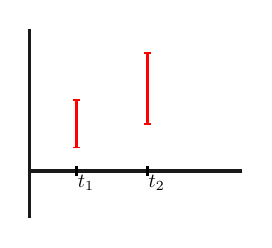
\begin{tikzpicture}[scale=0.6,transform shape]

\tikzset{
	pics/intervall/.style args={#1}{code={
	\draw[red,line width=0.3mm] (0,0) -- ++(0,#1) 
	node[rotate=90,sloped,inner xsep=0.8mm,inner ysep=0,pos=1,fill,red] (E) {}
	node[rotate=90,sloped,inner xsep=0.8mm,inner ysep=0,pos=0,fill,red] (E) {};
	},
	}
	}
        \tikzset{
          pics/tick/.style args={#1}{code={
            \draw[line width=0.3mm,inner sep=0mm] (0,-#1) -- (0,#1) ;
            },
          }
        }
          \tikzset{
            cross/.pic ={
              \draw[pic actions,rotate=#1,line width=0.3mm]
                (-3.5pt,0) -- (3.5pt,0)
                (0,-3.5pt) -- (0,3.5pt);
            },
          }
		  \draw  (1,0.5)  pic {intervall={1}} ;
		  \draw  (2.5,1)  pic {intervall={1.5}};

        \draw[black!90,line width=0.4mm] (0,-1) -- ++(90:4cm);
        %AXIS X
        \draw[black!90,line width=0.4mm] (0,0) --++(0:4.5cm); 
        \draw (1,0) pic[rotate=0] {tick={1mm}} node[yshift=-2.5mm,xshift=2mm,scale=1.2] {$t_1$} ;
        \draw (2.5,0) pic[rotate=0] {tick={1mm}} node[yshift=-2.5mm,xshift=2mm,scale=1.2] {$t_2$} ;
        %t1
        %\draw[red,line width=0.2mm] (1,0.5) -- (1,1.6);
        %\draw[orange] (1,1.5) pic {cross={45}} ;
        %\draw[blue] (1,0.5) pic {cross={45}} ;
        %t2
        %\draw[red,line width=0.2mm] (2,1) -- (2,1.6);
        %\draw[orange] (3,1) pic {cross={45}} ;
        %\draw[blue] (3,1.5) pic {cross={45}} ;
    \end{tikzpicture} 
    \hspace{5mm}
    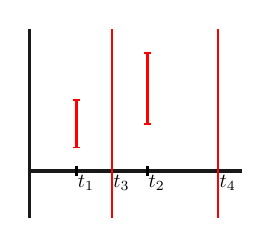
\begin{tikzpicture}[scale=0.6,transform shape]
		\tikzset{
	pics/intervall/.style args={#1}{code={
	\draw[red,line width=0.3mm] (0,0) -- ++(0,#1) 
	node[rotate=90,sloped,inner xsep=0.8mm,inner ysep=0,pos=1,fill,red] (E) {}
	node[rotate=90,sloped,inner xsep=0.8mm,inner ysep=0,pos=0,fill,red] (E) {};
	},
	}
	}
        \tikzset{
          pics/tick/.style args={#1}{code={
            \draw[line width=0.3mm,inner sep=0mm] (0,-#1) -- (0,#1) ;
            },
          }
        }
          \tikzset{
            cross/.pic ={
              \draw[pic actions,rotate=#1,line width=0.3mm]
                (-3.5pt,0) -- (3.5pt,0)
                (0,-3.5pt) -- (0,3.5pt);
            },
          }

		  \draw  (1,0.5)  pic {intervall={1}} ;
		  \draw  (2.5,1)  pic {intervall={1.5}};

        \draw[black!90,line width=0.4mm] (0,-1) -- ++(90:4cm);
        %AXIS X
        \draw[black!90,line width=0.4mm] (0,0) --++(0:4.5cm); 
        \draw (1,0) pic[rotate=0] {tick={1mm}} node[yshift=-2.5mm,xshift=2mm,scale=1.2] {$t_1$} ;
        \draw (2.5,0) pic[rotate=0] {tick={1mm}} node[yshift=-2.5mm,xshift=2mm,scale=1.2] {$t_2$} ;
        \draw (1.75,0) pic[rotate=0] {tick={1mm}} node[yshift=-2.5mm,xshift=2mm,scale=1.2] {$t_3$} ;
        \draw (4,0) pic[rotate=0] {tick={1mm}} node[yshift=-2.5mm,xshift=2mm,scale=1.2] {$t_4$} ;
        %t1
        %\draw[red,line width=0.2mm] (1,0.5) -- (1,1.6);
       % \draw[orange] (1,1.5) pic {cross={45}} ;
       % \draw[blue] (1,0.5) pic {cross={45}} ;
        %t2
        %\draw[red,line width=0.2mm] (2.5,1) -- (2.5,1.6);
       % \draw[orange] (2.5,1) pic {cross={45}} ;
        %\draw[blue] (2.5,1.5) pic {cross={45}} ;

        %t3
        \draw[red,line width=0.3mm] (1.75,-1) -- (1.75,3);
        %\draw[orange] (1.75,1.8) pic {cross={45}} ;
        %\draw[blue] (1.75,1) pic {cross={45}} ;

        %t4
        \draw[red,line width=0.3mm] (4,-1) -- (4,3);
        %\draw[orange] (4,1.8) pic {cross={45}} ;
        %\draw[blue] (4,1) pic {cross={45}} ;
    \end{tikzpicture} 
  \caption*{$B_1 \times B_2$ and $\pi_{J,J'}^{-1}(B_1 \times  B_2)$ for $J=\{t_1,\ldots,t_4\}$ and $J'=\{t_1,t_2\} $}  
\end{center}
\end{figure}
A family of consistent measures has the property that adding $E$s to a product does not change the measures corresponding to the increased time-set. We already know this situation from random vectors where we frequently used that 
\begin{align*}
	\P_{X_1}(1)=\P(X_1\in A)=\P(X_1\in A, X_2\in \R)=\P_{X_1,X_2}(A\times \R),
\end{align*}
which is nothing else but saying that the $1$-dimensional and $2$-dimensional marginals $\P_{X_1}$ and $\P_{X_1,X_2}$ are consistent. This is exactly what lies behind the lemma. If the finite dimensional distributions are defined through a "{}mother measures"{} $\P$ then adding time-points with no restriction is doing nothing.
\begin{proof}[Proof]
	Suppose that $J'$ has $n$ elements. We check the equality on a generator of the $n$-fold product $\sigma$-algebra, which are all products (boxes) made up from $n$ Borel-sets:
	\begin{align*}
		\P_{J'}(B_1\times \cdots \times B_n)
		\overset{\text{Def.}}&{=}\P(\{f:I\to E\,|\, f(t_i)\in B_i\, \forall t_i\in J'\})\\
		\overset{\text{do nothing}}&{=}\P\big(\{f:I\to E\,|\, f(t_i)\in B_i\, \forall t_i\in J', f(t_j)\in E\, \forall t_j\in J\backslash J'\}\big)\\
		\overset{\text{Def.}}&{=}\P_J \circ \pi^{-1}_{J,J'}(B_1\times\cdots \times B_n).
\end{align*}
%	\begin{figure}[h]
%		\begin{center}
%			\includegraphics[scale=0.15]{kolmogorov.jpeg}
%		\end{center}
%		\end{figure}
\end{proof}
Just as for distribution functions let us give a name to the characteristic property that holds for all finite dimensional martingals of a measures $\P$ on $\mathcal E^{\otimes I}$:
\begin{ldef}
	\begin{deff}
		A set of finite dimensional distributions $\{\P_J: |J|<\infty\}$ on $I$ is called \textbf{consistent} if $\P_J \circ \pi^{-1}_{J,J'}=\P_{J'}$ for all $J'\subseteq J$.
	\end{deff}
\end{ldef}
By the lemma consistency is a necessary property that must hold if there is a "mother"{} measure $\P$ behind. The amazing truth is that consistency alone is also sufficient for the existence of a "mother"{} measures as long as measurable space $(E,\mathcal E)$ is nice enough.
\begin{lsuperwichtigersatzExistence}
\begin{theorem}[Kolmogorov extension theorem]\label{Kolm}
	Let $E$ a Polish metric space, $\mathcal E=\mathcal B(E)$, and $I$ is an index set. If $\{\P^J:|J|<\infty\}$ is a family of consistent finite dimensional distributions on $I$, then there is a unique probability measures $\P$ on $\mathcal E^{\otimes I}$ such that $\P\circ \pi^{-1}_J=\P_J$ for all finite $J\subseteq I$.
\end{theorem}
\end{lsuperwichtigersatzExistence}
The importance of the theorem lies in the fact that finite dimensional distributions are easy (in many cases they are given by multivariate distribution functions or characteristic functions) whereas measures on infinite product spaces are not easy at all!\smallskip

Since the proof is lengthy let us first discuss one of the most important examples, the infinite product measures that was already claimed to exist in the proof of Theorem \ref{Folge}. To use the Kolmogorov extension theorem one only needs to write down a family of finite dimensional distributions and check they are consistent. But how should we do that without knowing the measures $\P$? This is very much in parallel to the construction of probability measures on $\mathcal B(\R)$. As an example, in order to prove the existence of uniformly distributed random variables we could already guess the distribution function $F_{\mathcal U([0,1])}$ and then check that it satisfies the defining properties needed. The approach is similar here:
\begin{ltipp}
	If a priori we have an idea on how (at least) the finite dimensional distributions of a measure $\P$ on $\mathcal E^{\otimes I}$ should look like then we can use that insight as an Ansatz to construct $\P$ through the Kolmogorov extension theorem.
\end{ltipp}
Here is an example of a situation in which the form of all finite dimensional distributions is a priori known.
\begin{ldef}
	\begin{deff}
		Suppose $(E, \mathcal E)$ is a measurable space and $\P$ is a probability measure on $\mathcal E$. Then a measures $\mu$ on $\mathcal E^{\otimes \N}$ is called an \textbf{infinite product measure} if the product formula
		\begin{align}\label{produkt}
			\mu(B_1\times\cdots \times B_n\times E\times E\cdots)=\P(B_1)\cdot ... \cdot \P(B_n)
		\end{align}
		holds for all $n\in\N$ and $B_i\in \mathcal E$. An infinite product measure is typically written as $\P^{\otimes \infty}$ or $\P^{\otimes \N}$.
	\end{deff}
\end{ldef}
Since $\P(E)=1$ the definition of the infinite product measures is already in  terms of all finite dimensional distributions that are needed for the construction.
\begin{llemma}
	\begin{theorem}
		If $E$ is a Polish metric space and $\P$ is a probability measure on $\mathcal B(E)$, then the infinite product measure $\P^{\otimes \infty}$ exists and is unique.
	\end{theorem}
\end{llemma}
\begin{proof}[Proof]
	\textbf{Uniqueness:} We already know the argument from finite product measures (compare the proof of Theorem \ref{Produktmass}). Since the righthand side of  \eqref{produkt} defines the measure on all finitely generated cylinder sets for $I=\N$ the measure is defined on a $\cap$-stable generator of $\mathcal B(E)^{\otimes \N}$. Hence, the uniqueness theorem for measures implies the uniqueness.\smallskip

	\textbf{Existence:} We already know from the definition that all finite dimensional marginals of $\P$ must be finite product measures of $\P$. Hence, we should apply the Kolmogorov extension theorem to the family $\{\P_J:|J|<\infty\}$, where $\P_J=\P^{\otimes |J|}$ for all finite subsets $J$ of $\N$. Of course those are consistent as all factors with $\P(E)=1$ can be taken out from the preimages $\pi^{-1}_{J,J'}(B_1\times \cdots \times B_{|J'|})$, for instance, 
	\begin{align*}
		\P_J(B_1\times E\times B_2\times \cdots \times B_3)&=\P(B_1)\cdot\P(E)\cdot \P(B_2)\cdot \P(E)\cdots \P(E)\cdot\P(B_3)\\
		&=\P(B_1)\cdot \P(B_2)\cdot \P(B_3)\\
		&=\P_{J'}(B_1\times B_2\times B_3).
	\end{align*}	
	Hence, there is a measure on $\mathcal B(E)^{\otimes \N}$ with the prescribed product measures as finite dimensional distributions. But this matches exactly the definition of the infinite product measures.
\end{proof}
The proof of the existence of infinite product measures finally completes the proof of Theorem \ref{Folge}. Now we really know that infinite sequences of independent random variables exist!

\marginpar{\textcolor{red}{Lecture 20}}

\begin{proof}[Proof of the Kolmogorov extension theorem]
	The uniqueness statement follows directly from Proposition \ref{lemma:unique}.\smallskip

	The basic idea of the proof is to apply the Carath\'eodory extension theorem. We will chose all finitely generated cylinder sets as the semiring $\mathcal S$ that generates the path $\sigma$-algebra and define a $\sigma$-additive set-function on $\mathcal S$ through the family of consistent finite dimensional distributions. The hard part will be to check the $\sigma$-additivity for which (as always) a compactness argument is needed. To carry out the compactness argument we essentially need to replace all appearing measurable sets by compacts sets while controlling the error that appears in the approximation. To carry this out two preliminary steps are needed.
	\begin{lstep}
		Every probability measure $\mu$ on the Borel-$\sigma$-algebra of a Polish metric space $(E,d)$ is inner regular, i.e. for all $B\in \mathcal B(E)$ there is a sequence of compact sets $K_n\subseteq B$ such that $\lim_{n\to\infty}\mu(B\backslash K_n)= 0.$
	\end{lstep}

	Recall from the proof of Proposition \ref{prop_4120} the set $A \coloneqq \bigcap_{n=1}^{\infty} \bigcup_{k=1}^{N_n}B_{\frac{1}{n}}(x_k) \in\cB(E)$. Since $A$ is totally bounded it's closure (which is also totally bounded) is compact. Defining $K$ to be the closure of $A$  we have already proved that $\mu(E\backslash K)\leq \varepsilon$. For $C$ closed we only need to define $K_C:=K\cap C$. Then $K_C$ is compact (closed and totally bounded) and $\mu(C\backslash K_C)=\mu(((E\backslash K)\cap C)\leq \mu(E\backslash K)\leq \varepsilon$. Hence, all closed sets are inner regular, their measure can be approximated by measures of compact subsets. Now we can use the trick of good sets. Define 
	\begin{align*}
		\mathcal M=\{B\in \mathcal B(E): B\text{ is inner regular}\}.
	\end{align*}
	It is not hard to see that $\mathcal M$ is a Dynkin system. If $B_1,...$ are disjoint, then chose $K_n\subseteq B_n$ compact such that $\mu(B_n\backslash K_n)\leq \frac{\varepsilon}{2^n}$. Then the ..................
	
	
	
	
	\footnote{An einem regnerischen tag aus-x0-en. heute regnets, dann der naechste kalte regnerische Tag.}. Since the closed sets $\mathcal C$ generate $\mathcal B(E)$ we can finish the argument as always:
	\begin{align*}
		\mathcal B(E)=\sigma(\mathcal C)  \overset{\ref{Hauptsatz}}{=}d(\mathcal C)\subseteq d(\mathcal M)=\mathcal M \subseteq \mathcal B(E).
	\end{align*}
	Hence, all measurable sets are inner regular. 
%	Since $E$ is separable for any $n\in \N$ there is a sequence $(x^n_k)_{k\in\N}$ such that $E=\cup_{k=1}^\infty B_{1/n}(x^n_{1/k})$ and by $\sigma$-additivity there exists an $I_n$ such that 
%	\begin{align*}
%		\P\Big(\Bigcup_{k=1}^{I_n}B_{1/n}(x^n_k)\Big)\geq 1-\frac{\varepsilon}{2^n}.
%	\end{align*}
%	We know this from .... Then the set $K:=\cap_{n=1}^\infty \cup_{k=1}^{I_n} B_{1/n}(x^n_k)$ is closed and
%	\begin{align*}
%		\P(K^c)=\P(\cup_{n=1}^\infty \cap_{k=1}^{I_n} B^c_{1/n}(x^n_k))\leq \sum_{n=1}^\infty \frac{\varepsilon}{2^n}\leq \varepsilon.
%	\end{align*}
%	Since $K\subseteq \cup_{k=1}^{I_n} B_{1/n}(x_k^n)$ for all $n$ we find that $K$ is totally bounded. Since $E$ is complete, $K$ is compact. 
The inner regularity of probability measures can now be used in a special situation where we replace "growing"{} sequences of Borel sets by growing sequences of compact sets:
\begin{lstep}
	Let $B_n\subseteq E^n$ a sequence of Borel sets such that $B_{n+1}\subseteq B_{n}\times E$, and $\mu_n$ a consistent sequence of measures on $\mathcal B(E)^{\otimes n}$, i.e. 
	\begin{align*}
		\mu_n(A_1\times\cdots \times A_{n-1}\times \R)=\mu_{n-1}(A_1\times \cdots \times A_{n-1}).		
	\end{align*}	
	If $\mu_n(B_n)>\varepsilon$ for all $n\in\N$, then there is a sequence of compact sets $K_n\subseteq B_n$ so that
		\begin{itemize}
			\item $K_{n+1}\subseteq K_n\times\R$,
			\item $\mu_n(K_n)\geq \frac{\varepsilon}{2}$ for all $n\in\N$.
		\end{itemize}
\end{lstep}
The claim essentially states that without loss of generality we will later be allowed to assume that all appearing measurable sets are compact sets.
\begin{figure}[h]
	\begin{center}
		\includegraphics[scale=0.13]{Kolmogorov2.jpeg}
		\caption*{More sequences through blue than black restrictions}
	\end{center}
	\end{figure}
In principle the idea is simple. Approximate all $B_n$ with a smaller compact $K_n$ and that's it. We just need to be careful since each $K_n$ gives an approximation error of $\epsilon$ so the error of their combination will add up in $n$. That's why we approximate finer and finer so that the sum of the approximation errors is $\varepsilon$. It is not surprising how to proceed: Chose compact $K_n^*\subseteq \R^n$ such that $K_n^*\subseteq B_n$ and $\mu_n(B_n\backslash K_n^*)\leq 
\frac{\varepsilon}{2^{n+1}}$ and then define
	\begin{align*}
		K_n=(K_1^*\times \R^{n-1})\cap ...\cap (K^*_{n-1}\times \R)\cap K_n^*.
	\end{align*}
	We only need to check that $K_n$ does the job. It follows directly that $K_n\subseteq B_n$ and $K_{n+1}\subseteq K_n\times \R$ and also that
	\begin{align*}
		\mu_n(K_n)\overset{\sigma\text{-add.}}&{=}\mu_n(B_n)-\mu_n(B_n\backslash K_n)\\
		&=\mu_n(B_n)-\mu_n(B_n\backslash ((K_1^*\times \R^{n-1})\cap ...\cap (K^*_{n-1}\times \R)\cap K_n^*))\\
		\overset{\sigma\text{-add.}}&{\geq} \mu_n(B_n)-\mu_n(B_n\backslash(K_1^*\times \R^{n-1}))-...-\mu_n(B_n\backslash K_n^*)\\
		\overset{B_k\subseteq B_1\times \R^{k-1}}&\geq \mu_n(B_n)-\mu_n(B_1\times \R^{n-1}\backslash K_1^*\times \R^{n-1})-...-\mu_n(B_n\backslash K_n^*)\\
		\overset{\text{consistent}}&\geq \mu_n(B_n)-\mu_1(B_1\backslash K_1^*)-...-\mu_n(B_n\backslash K_n^*)\\
		&\geq \varepsilon-\frac{\varepsilon}{4}-...-\frac{\varepsilon}{2^{n+1}}
		\geq \frac{\varepsilon}{2}.
	\end{align*}
That's it. Before we proceed let us quickly recall Carath\'eodory's extension Theorem \ref{KarlTheodor}:	
	\begin{ltipp}
	If $\mu$ is a $\sigma$-additive set-function on a semiring $\mathcal S$, then there is a unique measures $\bar \mu$ on $\sigma(\mathcal S)$ with $\mu(A)=\bar \mu(A)$ for all $A\in \mathcal S$.
	\end{ltipp}
	We proceed in two main steps. First, a semiring $\mathcal S$ and a set-function $\mu$ are defined which is shown to be well-defined. Secondly, the properties of a $\sigma$-additive set function are checked. We define $\mathcal S$ as the set of all finitely generated cylinder sets, so all sets $C$ that can be written as $\pi^{-1}_J(B_1\times \cdots\times B_n)$ for some finite subset $J=\{t_1,...,t_n\}$ of $I$ and Borel sets $B_i$. The set of finitely generated cylinder sets is clearly a semiring. The set function $\mu$ on $\mathcal S$ is defined as 
	\begin{align}\label{eq_22}
		\mu\big(  \pi^{-1}_J(B_1\times \cdots\times B_n)  \big):=\mathbb{P}_{J}(B_1\times\cdots\times B_n)
	\end{align}
	for all cylinder sets from $\mathcal S$. We now come to the main step of the argument:
	\begin{lstep}
		$\mu$ is a well-defined $\sigma$-additive set-function on $\mathcal S$.
	\end{lstep}
	\textbf{(i) $\mu$ is well-defined}: Suppose a cylinder set $C$ from $\mathcal S$ has two representations 
	 \begin{align}\label{eq_27}
			\pi^{-1}_{J}(B_1\times \cdots \times B_n)=C=\pi^{-1}_{\tilde J}(\tilde B_1\times \cdots \times \tilde B_m)
	\end{align}
	which can happen if some of the $B_i$ or $\tilde B_i$ are equal to $E$. It is precisely the assumed consistency property (we can cross out all $E$ and delete the time-points) that ensures that the measures of both representations is equal.\smallskip

	\textbf{(ii)} \textbf{$\mu$ is a $\sigma$-additive set-function}: There are two properties to check. We start with the empty set.  Since $\mu$ is well-defined we are allowed to write $\emptyset$ in some arbitrary way as a finite cylinder set: $\emptyset = \pi^{-1}_t(\emptyset)$ for arbitrary $t\in I$ yields $\mu(\emptyset)=\P_{\{t\}}(\emptyset)=0$.

		\smallskip The difficulty is to prove the $\sigma$-additivity of $\mu$ on $\mathcal S$. Assume $C_n$ is a sequence of disjoint cylinder sets from $\mathcal S$ such that $C:=\cupdot_{k=1}^\infty C_k\in \mathcal S$. We have to prove that $\mu(C)=\sum_{k=1}^\infty \mu(C_k)$. If we write 
\begin{align*}
	\mu(C)=\mu\big(C\,\backslash \cupdot_{k=1}^N C_k\big)+\mu\big(\cupdot_{k=1}^N C_k\big)
\end{align*}
and apply monotonicity of measures it is clear that it suffices to prove 
\begin{align}\label{lim:D}
	\lim_{N\to\infty}\mu(D_N)=0,
\end{align}
where $D_N=C\,\backslash \cupdot_{k=1}^N C_k\in \mathcal S$. To prove \eqref{lim:D} we use a compactness argument based on the steps above. The sequence $\mu(D_N)$ is decreasing (monotonicity of measures) to some number $\varepsilon$. Let us assume $\varepsilon>0$ and construct a contradiction. The contradiction will be that 
\begin{align}\label{contradiction}
	\cap_{N=1}^\infty D_N\neq \emptyset
\end{align}
which is absurd because as it would contradict $C=\cupdot_{k=1}^\infty C_k$. Since all $D_N$ are (finite) cylinder sets, also $D:=\cup_{N=1}^\infty D_N$ is a countable cylinder set for some times $t_1<t_2<...$. Since the $D_N$ decrease, without loss of generality (otherwise add artificially extra points with corresponding Borel-set $E$ that have no effect) we can assume that $D_N$ is finitely generated by more and more time-points:
\begin{align*}
	D_N=\{f: (f(t_1),..., f(t_N))\in B_N\}
\end{align*}
for a sequence of Borel sets $B_N\subseteq \mathcal E^N$ satisfying $B_{N+1}\subseteq B_{N}\times E$. Now we apply the regularity from the step above and replace without loss of generality the sets $B_N$ by compact sets $K_N\subseteq B_N$ (changing $\varepsilon$ into $\varepsilon/2$). Since the $K_N$ are non-empty (they have positive measures), we can pick vectors $x^N=(x_1^N,...,x_N^N)\in K_N$. The decreasing property of the $K_N$ implies that the sequences $(x_1^N)$ lies in the compact set $K_1$. Hence, there is a convergent subsequence $(x_1^{N_k})$ that converges to some $x_1\in K_1$. Next, the sequence $(x_1^{N_k}, x_2^{N_k})$ is contained in $K_2$, thus, there is another converging subsequence $(x_1^{N_k'}, x_2^{N_k'})$ that converges to some $(x_1,x_2)\in K_2$. Continuing like that we obtain a sequence $(x_n)$ in $E$ such that $(x_1,x_2,...,x_n)\in K_n\subseteq B_n$ for all $n\in\N$. But then the set of functions passing through $x_k$ at times $t_k$ are in all $D_N$. Hence, \eqref{contradiction} is matched and we have our contradiction.
\end{proof}



\subsubsection{(C) Path valued random variables and stochastic processes}
The third step in the triology of measure theory is to understand the connection of stochastic processes and path-valued random variables. We start with the natural generalization of Proposition \ref{zweiInterpr}:
\begin{llemma}
\begin{prop}\label{zweiInterprb}
		$X=(X_t)_{t\in I}$ is an $E$-valued stochastic process on $(\Omega, \mathcal A, \P)$ if and only if the mapping $$X:\omega\mapsto \big(t\mapsto X_t(\omega)\big)$$ is a path-valued random variable.
	\end{prop}
\end{llemma}
A bit of care is needed to explain the statement. If $(X_t)$ is a family of random variables it is clear how the path-valued mapping has to be interpreted. Fix $\omega$ and then consider all values $X_t(\omega)$ as a function in $t$. The converse is a bit more tricky. To switch back from the path-valued valued mapping to a family of $E$-valued mappings one needs to evaluate $X$ at all times $T$, formalized using the projections: $X_t:=\pi_t\circ X$. 
\begin{proof}[Proof]
	\begin{itemize}
		\item["$\Leftarrow$":] 
		For $B \in \mathcal E$ we have 
\[ X_t^{-1} (B) = X^{-1}(\pi_t^{-1}(B)) \in \mathcal A, \]
because $\pi_t^{-1}(B)$ is a finitely generated cylinder set and $X$ is $(\mathcal A, \mathcal E^{\otimes I})$-measurable.
		\item["$\Rightarrow$":] Using Proposition \ref{S2} the measurability property only needs to be checked on an arbitrary generator. We use the cylinder sets $\pi_t^{-1}(B)$ generated by single time-points:
		\begin{align*}
			X^{-1}(\pi_t^{-1}(B)) =\{\omega \in \Omega: X_t(\omega)\in B\}=X^{-1}_t(B)\in \mathcal A.
		\end{align*}
		Hence, seen as a path-valued random variable $X$ is measurable.
	\end{itemize}
\end{proof}
Next, the notion of the law from random variables and random vectors is generalized to stochastic processes:
\begin{ldef}
\begin{deff}\label{def:SP}
		Suppose $X$ is an $E$-valued stochastic process on $(\Omega, \mathcal A, \P)$. 
		\begin{enumerate}[label=(\roman*)]
			\item The image measure 		
		\begin{align*}
			\P_X(A):=\P(X\in A),\quad A\in \mathcal E^{\otimes I},
		\end{align*}
		is called the \textbf{law of $X$}.
		\item For a finite subset $J=\{t_1,...,t_n\}$ of $I$ the law evaluated on the cylinder sets spanned by $J$
		\begin{align*}		
			\P_X^{J}(B_1\times ...\times B_n)&:=\P(X_{t_1}\in B_1,..., X_{t_n}\in B_n)\\
			&=\P_X(\pi_{t_1,...,t_n}^{-1}(B_1\times ... \times B_n)),\quad t_i\in I, B_i\in \mathcal E,
		\end{align*}
		is called a \textbf{finite dimensional distribution of $X$}.
	\end{enumerate}
\end{deff}
\end{ldef}
Warning! The law of a stochastic process is a delicate object, a measure on the path space. Usually the law does not play a big role and we are mostly interested in the finite dimensional distributions. Both concepts are essentially equivalent but finite dimensional distributions are laws on much nicer $\sigma$-algebras.
\begin{llemma}
\begin{prop}
		The law of a stochastic process is uniquely determined by the family of all finite dimensional distributions.
\end{prop}
\end{llemma}
\begin{proof}[Proof]
	This follows from the abstract theory of the previous section. Since all finitely generated cylinder sets generate the path $\sigma$-algebra $\mathcal E^{\otimes I}$ and are intersection stable the measure $\P_X$ is uniquely determined on all sets $\pi_{t_1,...,t_n}^{-1}(B_1\times \cdots \times B_n)$.
\end{proof}
It is crucial to assume that \textbf{all} finite dimensional distributions are equal. If $X$ is a symmetric random variable, then $(X,-X)$ and $(X,X)$ have different laws but the same one-dimensional distributions.
\begin{ldef}
\begin{deff}
	Two stochastic processes $X$ and $Y$ with index set $I$ have the same law if $\P_X=\P_Y$. Equivalently, we say they have the same finite-dimensional distributions if $\P_X^J=\P_Y^J$ for all finite $J\subseteq I$.
\end{deff}
\end{ldef}
Just as for random variables, the case $|I|=1$, two stochastic processes with same law do not need to be defined on the same probability space. The notion of equality in law is the weakest equality notation available, stronger notions will be discussed in the next section. \smallskip

If you remember well the previous 300 pages of these lecture notes you will know what is up next. The existence of stochastic processes using the canonical constructions. Earlier versions covered the cases $|I|=1$, $|I|<\infty$, and $I=\N$. Here is the general version for arbitrary $I$ only assuming $E$ is Polish.
\begin{lsuperwichtigersatzExistence}
	\begin{theorem}[Canonical construction on $E^{I}$]\label{KolmogorovProcess}
		Suppose $E$ is a Polish metric space, $I$ an index set, and $\{\P_J:|J|<\infty\}$ a consistent family of finite-dimensional distributions. Then there is a stochastic process $X$ on some probability space $(\Omega, \mathcal A, \P)$ with marginals $\P_X^J=\P_J$ for all finite sets of times.
	\end{theorem}
\end{lsuperwichtigersatzExistence}
\begin{proof}[Proof]
	In the usual way we construct a probability space and a (path-valued) random variable:
	\begin{itemize}
		\item $\Omega=E^I$
		\item $\mathcal A=\mathcal E^{\otimes I}$
		\item $\P=\P_X$, the measure on $\mathcal E^{\otimes I}$ obtained from the consistent family using Theorem \ref{Kolm}.
		\item $X$ is the identity mapping from $E^I$ to $E^I$.
		\item $X_t=\pi_t(X)$ the evaluation of $X$ at time $t$.
	\end{itemize}
	The measurability of $X$ is clear (preimages of measurable sets are the same measurable sets) and the law is $\P_X=\P$ which has the good finite dimensional distributions by construction.
\end{proof}
People tend to like the canonical construction as it always works (justifying the name canonical) but there are very good reasons to avoid the canonical construction if possible. For instance the statement "{}$X$ is $\P$-almost surely continuous/differentiable/constant/etc."{} is problematic for a real-valued process on the canonical probability space because such events are not measurable in $\mathcal B(\R^{[0,\infty)})$, hence, no probabilities can be defined. In fact, the problem can be avoided using a better definition of nullsets than the one we gave in Definition \ref{def:Nullmenge}, compare also the footnote after the definition.
\begin{lwarnhinweis}
	From now on a set $A\subseteq\Omega$ is called a nullset if there is a measurable set $B$ with $A\subseteq B$ and $\P(B)=0$. A property $E$ holds $\P$-almost surely, if $\{\omega: E(\omega) \text{ does not hold}\}$ is contained in a measurable set with measure $0$.
\end{lwarnhinweis}
There is no problem for the earlier discussion as all previous nullsets of interest $\{X=Y\}$, $\{X\geq 0\}$, $\{X_n \text{ converges}\}$, etc. are measurable themselves. We will return a few times to the measurability problems on the path space but now want to get towards examples. Here is a first important class of stochastic processes that can be constructed using the theory developed above.
%\begin{example}[iid sequences of random variables]
%	Suppose $E$ is a Polish metric space, $\P$ is a distribution on $(E,\mathcal B(E))$, and suppose $I=\N$. Then define for all natural numbers $t_1<...<t_n$ the finite product measures
%	\begin{align*}
%		\P^{t_1,...,t_n}(B_1\times \cdots \times B_n):=\P(B_1)\cdot... \cdot \P(B_n),\quad B_i\in \mathcal E.
%	\end{align*}
%	Since $\P(E)=1$ it follows immediately that the family is consistent:
%	\begin{align*}
%		\P^{t_1,...,t_{n+1}}(B_1\times \cdots \times B_n\times E)=\P(B_1)\cdot... \cdot \P(B_n)\cdot \P(E)=\P^{t_1,...,t_{n}}(B_1\times \cdots \times B_n).
%	\end{align*}
%	Hence, there is a stochastic processes $X$ indexed by $\N$ with finite dimensional distributions $\P^{t_1,...,t_n}$. What does this mean? If we interpret the stochastic process $(X_t)_{t\in\N}$ as a family (here: sequence) of random variables $X_1,X_2,...$ then  
%	\begin{align*}
%		\P(X_1\in B_1,..., X_n\in B_n)&=\P^{1,...,n}_X(B_1\times \cdots \times B_n)\\
%		&=\P(B_1)\cdot ... \cdot \P(B_n)\\
%		&=\P_X^{1} (B_1)\cdot ... \cdot \P_X^{n}(B_n)=\P(X_1\in B_1)\cdot ...\cdot \P(X_n\in B_n).
%	\end{align*}
%	This means we constructed a sequence of iid $E$-valued random variables with prescribed distribution $\P$.
%\end{example}
\begin{ldef}
	\begin{deff}
		A stochastic process $(X_t)_{t\in I}$ is called a \textbf{Gaussian process} if all finite dimensional distributions are multi-variate Gaussian. We call $$m(t):=\E[X_t],\quad t\in I,$$ the mean-function of $X$ and $$K(t,s):=\E[(X_t-m(t))(X_s-m(s))],\quad t,s\in I,$$ the covariance function of $X$. A Gaussian process is called \textbf{centered} if $m\equiv 0$.
	\end{deff}
\end{ldef}
Chosing $I=\{1,...,d\}$ shows that Gaussian processes are direct generalizations of Gaussian vectors and in this case $m$ is the mean-vector and $K$ the covariance matrix. Covariance functions are symmetric and positive semi-definite, i.e.
\begin{align*}
	\sum_{i,j=1}^na_ia_jK(t_i,t_j)&=\sum_{i,j=1}^n a_ia_j \E[(X_{t_i}-m(t_i))(X_{t_j}-m(t_j))]\\
	&=\E\Big[\Big(\sum_{i=1}^n a_i(X_{t_i}-m(t_i))\Big)^2 \Big]\geq 0,
\end{align*}
for all $n\in\N$, $t_i, t_j\in I$ and $a_i\in \R$. Note that in the case $I=\{1,...,d\}$ this is exactly the definition of a positive semi-definite matrix. Here are some examples for symmetric  positive semi-definite functions on $I=[0,\infty)$:
\begin{align*}
	K(t,s)=t\wedge s, \quad K(t,s)=\exp(|t-s|),\quad K(s,t)=(1+|t-s|^2)^{-\alpha},\,\alpha\geq 0.
\end{align*}
	Gaussian processes are particularly useful as they are easy to construct through Kolmogorov's extension theorem:
\begin{luebung}
	Let $m:I\to \R$ and $K:I\times I\to \R$ be symmetric and positive semi-definite. Then there is a Gaussian process $(X_t)_{t\in I}$ with mean-vector $m$ and covariance function $K$.\smallskip

	Hint: In order to use Theorem \ref{KolmogorovProcess} one has to write down all finite dimensional distributions. Just as in the construction of infinite product measures we have the advantage that those are already known, as they are supposed to be multivariate Gaussian. Go back to the end of Section \ref{sec:applications} to see why only $m$ and $K$ are needed to guess the form of all finite dimensional distributions and then show that they are consistent.
\end{luebung}
A further nice application of the construction theorem is to construct Markov chains on a infinite time-horizon:
\begin{luebung}
	Use Theorem \ref{KolmogorovProcess} to construct a Markov chain $(X_t)_{t\in\N}$ on a finite state-space $\{1,...,n\}$ with transition matrix $P$.
\end{luebung}


\subsection{Stochastic processes with continuous sample paths}
\marginpar{\textcolor{red}{Lecture 21}}

So far we developed a tool to construct stochastic processes with given finite-dimensional distributions using the canonical construction based on the Kolmogorov extension theorem. The story is not over, yet, if we are interested in stochastic processes with regular (e.g. continuous) sample paths. One of the motivations to keep the weak convergence chapter more general than just $\R^d$ was to introduce a notion of convergence of stochastic processes. In order to do so we must be able to interpret a stochastic process as a random variable with values in a Polish space. So far, it is unclear what that Polish space could be used because the generic path space $\R^{I}$ has no topological structure what so ever. The aim of this section is two-fold. First, we first explain the path-space of continuous real-valued functions and stochastic processes with continuous paths, secondly, we discuss ways of constructing such processes. Unfortunately, it's not possible to prove a generic construction theorem like the Kolmogorov extension theorem, the proof of the Kolmogorov extension theorem breaks down if used on continuous functions. Instead, we will introduce a method to modify stochastic processes without path regularity into processes with (H\"older) continuous processes. 

\subsubsection{The path space of continuous functions}
The space of continuous functions on a compact set (here: compact interval) has already been studied in the previous chapter. It is well-known from basic analysis that $C([0,T])$ is complete, the Stone-Weierstra\ss{} theorem applied to polynomials with rational coefficients also shows that $C([0,T])$ is separable. Hence, $(C([0,T]), ||\cdot ||_\infty)$ is a Polish space and as such suitable for the theory developed in the previous chapter. As we are mostly interested in stochastic processes indexed by $[0,\infty)$ it is important to see that also continuous functions indexed by $[0,\infty)$ can be made into a Polish space:
\begin{llemma}
\begin{prop}
	\begin{enumerate}[label=(\roman*)]
		\item If we define
			\begin{align*}
				d(f,g)\coloneqq \sum_{k=1}^{\infty} \frac{d_k(f,g)}{2^k},\quad d_k(f,g) = \sup_{x\in [0,k]} \lvert f(x) - g(x)\rvert \wedge 1,
			\end{align*}
		then $d$ is a metric on $C([0,\infty))$. 
		\item $d$ metrizes convergence on compacts, that is
		\begin{align*}
			\lim_{n\to\infty} d(f_n,g)=0\quad \Leftrightarrow \quad \lim_{n\to\infty}\sup_{x\in K}|f_n(x)-g(x)|=0\text{ for all }K\text{ compact.}
		\end{align*}
		\item $( C([0,\infty)),d )$ is a Polish metric space.
	\end{enumerate}
\end{prop}
\end{llemma}
The truncation by $1$ is important for two reasons. First, it ensures the metric is always finite, and secondly, it allows to use dominated convergence in the proof below.
\begin{proof}[Proof]
(i)	We know from basic analysis that $d_k$ is a metric on $C([0,k])$, the properties of a metric space then follow immediately for $d$.\smallskip

(ii) It follows from the Heine-Borel Theorem that all compact subsets of $[0,\infty)$ are bounded. \smallskip
		
		"$\Rightarrow$": Suppose $\lim_{n\to\infty} d(f_n,g)=0$. Chose $K$ compact and some $k$ such that $K\subseteq [0,k]$. Since $\frac{d_k(f_n,g)}{2^k}\leq d(f_n,g)$ we find $\lim_{n\to\infty}\sup_{x\in K}|f_n(x)-g(x)|\leq \lim_{n\to\infty}d_k(f_n,g)=0$.\smallskip
	
		"$\Leftarrow$": The truncation by $1$ allows us to apply the dominated convergence theorem to get
		\begin{align*}
			\lim_{n\to\infty}d(f_n,g) \overset{\text{DCT}}{=} \sum_{k=1}^{\infty} \lim_{n\to \infty} d_k(f_n,g)\frac{1}{2^k}=0,			
		\end{align*}
			since all $[0,k]$ are compact.\smallskip

		 (iii) Separability: The set of polynomials restricted to $[0,n]$ with rational coefficients is countable and dense in $( C([0,n]),||\cdot||_\infty)$, see the discussion below Theorem \ref{Weierstrass_approx}. A diagonal argument then shows that all polynomials with rational coefficients are countable and dense in $(C([0,\infty)), d \big)$. Hence, the separability is proved.\smallskip
		
		Completeness: Suppose $(f_n)_{n\in\mathbb{N}}$ is Cauchy. By the definition of the metric, $(f_n)_{n\in\mathbb{N}}$ restricted to $[0,k]$ is also Cauchy in $(C([0,k]),||\cdot||_\infty)$. Since $( C([0,k]), ||\cdot||_\infty)$ is complete, for all $k\in\N$ there is a uniform (continuous) limit $g_k$ on $[0,k]$. Let us define a function $g:[0,\infty)\to \R$ as $g_k(x)$ for $x\in [0,k]$ and some $k>x$. Since $g_k = g_{k'}$ on $[0,k]$ for all $k' \geq k$ this construction is well-defined. Using dominated convergence once more yields
		\begin{align*}
			\lim_{n\to\infty}d(f_n,g) \overset{\text{DCT}}{=} \sum_{k=1}^{\infty} \lim_{n\to\infty} d_k(f_n,g)\frac{1}{2^k} = 0.
		\end{align*}
		Hence, $( C([0,\infty)),||\cdot||_\infty)$ is complete.
\end{proof}
Since $\big( C([0,\infty)),d \big)$ is a Polish metric space there is a natural $\sigma$-algebra on $E$, the Borel-$\sigma$-algebra generated by all open sets. Such a $\sigma$-algebra has much more structure than the product $\sigma$-algebra on the generic path space $\R^{[0,\infty)}$. As an example, all probability measures are inner regular. In contrast, $\mathbb{R}^{[0,\infty)}$ is topologically nothing useful. That's why the $\sigma$-algebra is not the topological $\sigma$-algebra induced by open sets (what are open sets without a topology?) but defined "by hands". Even though $\cB(C([0,\infty)))$ is structurally much more rich there is a lot of similarity to the generic path $\sigma$-algebra. For example both $\sigma$-algebras have the same simple generators, the cylinder sets, but now cylinder sets of continuous functions.
\begin{llemma}
\begin{prop}
	$\cB ( C([0,\infty)))$ is generated by the cylinder sets of continuous functions, i.e. 
	\begin{align*}
		\cB \big( C([0,\infty))\big) &= \sigma( \{\pi_t^{-1}(B):t \geq 0, B\in  \mathcal B(\R) \}),\\
				&= \sigma \big( \{ \text{finitely generated cylinder sets of continuous functions} \}\big),
	\end{align*}
	where $\pi_t:C([0,\infty))\to \R, f\mapsto f_t,$ are the projections on time $t$.
\end{prop}
\end{llemma}
In order to avoid confusion with the product $\sigma$-algebra on all generic functions let us emphasize the difference of projections on all continuous functions and generic functions. 
\begin{figure}[h]
	\begin{center}
		\includegraphics[scale=0.07]{box7.jpeg}
		\caption*{cylinder sets of continuous and all functions}
	\end{center}
\end{figure}
The cylinder sets of all functions are much larger since they contain all continuous functions passing through $B$ at time $t$ but also such discontinuous functions.
\begin{proof}[Proof]
	Intersecting cylinder sets generated by a single time-point leads to all finitely generated cylinder sets. Hence, the second equality holds and we only need to check the first. We will use the typical trick that in order to show $\sigma(\cE)=\sigma(\cE')$ it is enough to show $\cE\subseteq \sigma(\cE')$ and $\cE'\subseteq \sigma(\cE)$. To do so note that the projections $\pi_t:C([0,\infty))\to \R$ are continuous mappings. This follows immediately from the metric of $C([0,\infty))$. If $f_n\to f$, then the metric implies pointwise convergence $f_n(t)\to f(t)$ for all $t\in [0,\infty)$ which is nothing but $\pi_t(f_n)\to \pi_t(f)$. \smallskip


	"$\supseteq$"{}: Since the projections $\pi_t$ are continuous and we are working with Borel-$\sigma$-algebras they are also measurable. Hence, all preimages of $\pi_t$ (cylinder sets generated by one time-point) are in $\cB \big( C([0,\infty))\big)$.\smallskip
	
	"$\subseteq$"{}: It is enough to show that some generator of $\cB \big( C([0,\infty))\big)$ is contained in $\sigma(\{ \pi_t \colon t \geq 0 \})$. We chose the open sets. Since $(C([0,\infty)),d)$ is separable every open set can be written as a countable union of open balls (the open balls around polynomials with rational coefficients form a base of the topology). Hence, we need to show that open balls of functions are in $\sigma(\{ \pi_t \colon t \geq 0 \})$. Here is a trick. It is enough to prove that all mappings $f\mapsto d(f_0,f)$ are measurable as their preimages of $[0,\varepsilon)\in \mathcal B([0,\infty))$ are $B_{\varepsilon}(f_0)$. By the definition of $d$ it is enough to show that all $f\mapsto d_k(f_0,f)$ are measurable for all $k\in\N$ as limits, sums, scalar multiplications, and taking minima are operations that preserve measurability by Proposition \ref{hilf}. But this follows by rewriting
	\begin{align*}
		d_k(f_0,f) = \sup_{t\leq k} | f_0(t)- f(t) | \wedge 1
		= \sup_{t\leq k,\:t\in\mathbb{Q}} | f_0(t)- f(t) | \wedge 1 
		= \sup_{t\leq k,\:t\in\mathbb{Q}} | \pi_t(f_0) - \pi_t(f) | \wedge 1,
	\end{align*}
	since the righthand side is a concatenation of measurable functions with measurable operations.
\end{proof}
The previous proposition shows that $\cB \big( C([0,\infty))\big)$ has the same type of generator as the product $\sigma$-algebra $\mathcal E^{\otimes I}$ on $E^I$. It is thus reasonable to copy ideas carried out before. If $J\subseteq [0,\infty)$ is a finite set with $n$ time-points, then
\begin{align*}
	\P_J(B_1\times \cdots B_{n}):= \P(\{f\in C([0,\infty)): f(t_1)\in B_1,... ,f(t_n)\in B_n\}),\quad B_i\in \mathcal B(\R),
\end{align*}
is called a finite dimensional distribution of $\P$. Since probability measures are uniquely defined on a $\cap$-stable generator the finite dimensional distributions uniquely determine the law, just as Proposition \ref{lemma:unique} for probability measures on the generic path space.
\begin{llemma}
\begin{prop}
	A probability measure $\P$ on $\cB( C([0,\infty)))$ is uniquely determined by the family $\{\P_J: |J|<\infty\}$ of all finite dimensional marginal distributions.
\end{prop}
\end{llemma}
The generator of finitely generated cylinder sets reveals a striking fact. Restricting a cylinder set from the generator of $\mathcal B(\R^{[0,\infty)})$ to the continuous functions gives a cylinder set from the generator of $\cB( C([0,\infty)))$. This is no coincidence, the same holds for the entire $\sigma$-algebras:
%The very unpractical generic path space $( \mathbb{R}^{[0,\infty)},\cB(\mathbb{R})^{\otimes [0,\infty)} )$ and the nice continuous path space $( C([0,\infty)), \cB(C([0,\infty))) )$ are actually not so far apart. Seeing continuous function as a subset of all generic functions the nice continuous path $\sigma$-algebra is the "{}trace-$\sigma$-algebra"{} of the nasty generic path $\sigma$-algebra. 
\begin{llemma}
\begin{prop}
	$\mathcal B(\R^{[0,\infty)})_{|C([0,\infty))}=\cB \big( C([0,\infty))\big)$
\end{prop}
\end{llemma}
Recall that for a measurable space $(\Omega, \mathcal A)$ and some (possibly non-measurable) set $B\subseteq \Omega$ one defines the trace-$\sigma$-algebra on $B$ as $\mathcal A_{|B}:=\{A\cap B: A\in \mathcal A\}$. It is easy to check that this is again a $\sigma$-algebra and that $\mathcal C\cap B$ is a generator of $\mathcal A_{|B}$ if $\mathcal C$ is a generator of $\mathcal A$.
\begin{proof}[Proof]
	We use again the strategy from Example \ref{bsp:borel} that in order to prove equality $\sigma(\cE)=\sigma(\cE')$ it suffices to show $\cE\subseteq \sigma(\cE')$ and $\cE'\subseteq \sigma(\cE)$.\smallskip

	"{}$\subseteq$"{}: Note that the trace-$\sigma$-algebra is generated by all intersections of finitely generated cylinder sets of all functions with the continuous functions. Of course, all such sets are finitely generated cylinder sets of continuous functions (generated by the same time-points), which are in $\cB \big( C([0,\infty))\big)$.\smallskip

	"{}$\supseteq$"{}: We use the cylinder sets of continuous functions generated by one time-point. Those are of course the same as the cylinder sets of all functions (through the same time-point) intersected with the continuous functions. But those sets are in the trace-$\sigma$-algebra.
\end{proof}
Here is an important question that is motivated from the observation that $\cB \big( C([0,\infty))\big)$ and $\mathcal B(\R^{[0,\infty)})$ have the same kind of semiring generators.
\begin{ltipp}
If the continuous paths $\sigma$-algebra is so similar to the generic product $\sigma$-algebra, can we also use the Carath\'eodory extension theorem to construct a measure from a consistent family of finite dimensional distributions? The frustrating answer is: no!
\end{ltipp}
Going through the proof of the Kolmogorov extension theorem one finds that the proof fails in the very end when we constructed the contradiction. We stop the discussion here, there is no complete identification of all probability measures on $C([0,\infty))$. Nonetheless, we will see below how many stochastic processes with continuous sample paths can be constructed without the canonical representation.

\begin{ldef}
	\begin{deff}
		A stochastic process $(X_t)_{t\geq 0}$ on some probability space $(\Omega, \mathcal A, \P)$ is said to have continuous/differentiable/etc. paths if there is an event $C$ of probability $1$ so that $t\mapsto X_t(\omega)$ is continuous/differentiable/etc. for all $\omega \in C$.
	\end{deff}
\end{ldef}
It is important to note that the definition does not use that $\{\omega: t\mapsto X_t(\omega)\}$ itself is measurable, only that it contains a measurable set $C$ which has probability $1$.\smallskip

The law $\P_X(B):=\P(X\in B)$ of a stochastic process has already been defined on the product $\sigma$-algebra $\mathcal B(\R^{[0,\infty))})$, as a push-forward of the process seen as path-valued random variable (see Definition \ref{def:SP}). If $X$ has continuous sample paths it would certainly be nicer also to define the law of $X$ on the continuous functions. This can be done, with one little refinement. Since $t\mapsto X_t(\omega)$ is only known to be continuous for all $\omega\in C$ for some event $C$ of measure $1$ we first restrict the entire probability space to $C$. Then paths are continuous for all $\omega\in \Omega':=\Omega\cap C$ and the law can be defined:
\begin{ldef}
	\begin{deff}
		If $(X_t)_{t\geq 0}$ is a stochastic process with continuous sample paths then the law $\P_X$ of $X$ on $C([0,\infty))$ is defined as 
		\begin{align*}
			\P_X(B)=\P_{|C}(X\in B),\quad B\in \mathcal B(C([0,\infty)).
		\end{align*}
	\end{deff}
\end{ldef}
Since $C$ has full measure this little twist does not effect the finite dimensional distributions. The concept of the law of continuous processes will become much more important later when we prove the universal approximation property of a Brownian motion by random walks (Donsker's theorem). For now we only remark that any given probability measure $P$ on $\mathcal B(C([0,\infty))$ allows a canonical construction:
\begin{itemize}
	\item $\Omega:=C([0,\infty))$,
	\item $\mathcal A:=\mathcal B(C([0,\infty)))$,
	\item $\P:=P$,
	\item $X$ is the identity mapping from $C([0,\infty))$ to $C([0,\infty))$ and $X_t=\pi_t\circ X$.
\end{itemize}
\begin{luebung}
	Check that $(X_t)_{t\geq 0}$ is a continuous stochastic process on $(\Omega, \mathcal A, \P)$ with law $\P_X=P$.
\end{luebung}
The big trouble about continuous stochastic processes is that there is no generic construction theorem for probability measures on the continuous paths, hence, no generic construction theorem of continuous stochastic processes through the canonical construction. There are two major ways to overcome this problem: 
\begin{itemize}
	\item Some continuous stochastic processes can be written down explicitly.
	\item Some discontinuous stochastic processes can be modified into continuous processes.
\end{itemize}
For the first approach here is a simple example, a similar example appears later as one of two possible constructions of the Brownian motion.
\begin{example}
	Take an iid sequence $Y_1,Y_2,...$ on some probability space $(\Omega,\cA,\mathbb{P})$ (this is based on the Kolmogorov extension theorem!) and define the random walk with jump-sizes $Y$ as in Example \ref{ex:RW}. Now define $X$ to be the linear interpolation as in the illustration. 
	\begin{figure}[h]
		\begin{center}
			\includegraphics[scale=0.07]{RW.jpeg}
			\caption*{cylinder sets of continuous and all functions}
		\end{center}
	\end{figure}
	Then $t\mapsto X_t(\omega)$ is continuous even for all $\omega \in \Omega$. The corresponding law $\P_X$ on $C( [0,\infty))$ is called the \textbf{random walk law}. It will later be proved that random walk laws of scaled random walks converge weakly on $\mathcal B(C( [0,\infty) ))$ to the Wiener measures, the law of the Brownian motion.
\end{example}
We now turn to the powerful second approach, modifying discontinuous processes into continuous processes.
\subsubsection{The constructing of continuous stochastic processes}
There are different ways of defining the regularity of a real-valued functions. Continuity and differentiability are simple but not very precise notions, a more refined notion is H\"older continuity. 
\begin{ldef}
	\begin{deff}
		A function $f:\R^d\to\R$ is called H\"older-continuous of index $\gamma\in (0,1]$ 
		\begin{align*}
			|f(x)-f(y)|\leq K |x-y|^\gamma,\quad \forall x,y\in\R^d.
		\end{align*}
		A function $f$ is called locally H\"older continuous of index $\gamma>0$ if for all $x$ there is a neighborhood $U$ of $x$ and a constant $K_x$ such that 
		\begin{align*}
			|f(x)-f(y)|\leq K_x |x-y|^\gamma,\quad \forall y\in U.
		\end{align*}
	\end{deff}

\end{ldef}
The intuition should be that the roughness decreases for increasing $\gamma$ and $\gamma=1$ gives pretty smooth functions. Why is this? Suppose $x$ is close to $y$. Then the difference of the function between $x$ and $y$, also called an increment, is bounded by the distance raised to the power $\gamma$. If $x$ is very close to $y$ then increasing the power $\gamma$ decreases the size of the increment $|f(x)-f(y)|$, $f$ has infinitesimally small fluctuations (the spikes are not very sharp).
\begin{figure}[h]
	\begin{center}
		\includegraphics[scale=0.07]{rough.jpeg}
		\caption*{from rough to smooth: small $\gamma$, medium $\gamma$, $\gamma=1$}
	\end{center}
	\end{figure}
	To sharpen your intuition please think about the following exercise.
\begin{luebung}
	\begin{itemize}
		\item If $f$ is (locally) H\"older continuous of index $\gamma$, then $f$ is also (locally) H\"older continuous of index $\gamma'$ for all $\gamma'<\gamma$.
		\item If $f$ is continuously differentiable, then $f$ is locally H\"older continuous of index $1$ (which is the same as Lipschitz continuous).
		\item If $f$ is would be H\"older continuous with index $\gamma>1$, then $f$ must be constant. That's why we directly restrict to $\gamma\in (0,1]$.
		\item Polynomials $f(x)=|x|^\beta$, $\beta<1$, are not differentiable at $0$ but H\"older continuous of index $\beta$. Away from $0$ they are continuously differentiable, hence, locally Lipschitz continuous.
	\end{itemize}
\end{luebung}
Motivated by the last example we might think of H\"older continuous functions of index $\beta$ to be spiky functions with (possibly many) rough tips that can be as rough as $|x|^\beta$ around $0$.\smallskip

We will prove below that under certain conditions a stochastic process can be "modified"{} in a way that sample paths are continuous. Even better, there is a relatively simple condition under which sample paths are H\"older continuous with an identifiable index $\gamma$. Caused by the additional complexity of time there are different notions of equality of stochastic processes that go beyond the uniqueness of the laws when seen as a path-valued random variable. 
\begin{ldef}
	\begin{deff}
		Suppose $X$ and $Y$ are stochastic processes with index set $I$ on the same probability space $(\Omega, \mathcal A, \P)$. Then $X$ is a \textbf{modification} of $Y$ if $\P(X_t=Y_t)=1$ for all $t\in I$. 
	\end{deff}
\end{ldef}
Being modifications of each other is a very different concept of equality of processes than having the same finite dimensional distributions (i.e. same law). Here, $X$ and $Y$ must be defined on the same probability space and, intersecting events of probability $1$, $X$ and $Y$ automatically have the same finite dimensional distributions. In a way, being modifications of each other is much more equal than only having same law. Still, the paths of $X$ and $Y$ could be very different. As an example if all $X_t$ are symmetric random variables, then mirroring the path gives processes that look very different but $X$ and $-X$ are modifications of each other. The natural stronger notion would move "for all"{} in the probability. We want to call two processes indistinguishable if $\P(X_t=Y_t\text{ for all }t\in I)=1$. But there is a technical problem: Writing $\{X_t=Y_t\text{ for all }t\in I\}=\cap_{t\in I}\{X_t=Y_t\}$ there is again an uncountability problem. The righthand side is measurable if $I$ is countable, but not necessarily if $I$ is uncountable. Here is the good definition:
\begin{ldef}
	\begin{deff}
		Suppose $X$ and $Y$ are stochastic processes with index set $I$ on the same probability space $(\Omega, \mathcal A, \P)$. Then $X$ and $Y$ are called \textbf{indistinguishable} if there is an event $C$ with probability $1$ such that $X_t(\omega)=Y_t(\omega), t\in I,$ for all $\omega\in C$.
	\end{deff}
\end{ldef}
Here is the simplest example to separate both notions of equality for processes. Suppose $\mathcal U\sim \mathcal U([0,1])$ is a uniformly distributed random variable on some probability space $(\Omega, \mathcal A, \P)$ and define the stochastic processes $X_t:=0$ and $Y_t:=\mathbf 1_{\{U\}}(t)$ on $(\Omega, \mathcal A, \P)$ with index set $I=[0,1]$. Then $X$ is a modification of $Y$ as $\P(X_t=Y_t)=\P(U\neq t)=1$ but their paths are almost surely different.
\begin{figure}[h]
	\begin{center}
		\includegraphics[scale=0.07]{unique.jpeg}
		\caption*{modifications but not indistinguishable}
	\end{center}
	\end{figure}

Please check the connections of the equalities for processes and think about simple counter examples:
\begin{luebung}
	Let
	\begin{enumerate}[label=(\roman*)]
		\item $X$ and $Y$ are indistinguishable.
		\item $X$ is a modification of $Y$.
		\item $X$ and $Y$ have the same finite dimensional distributions (and same law).
	\end{enumerate}
	Show that (i)$\Rightarrow$(ii)$\Rightarrow$(iii) but both converse implications are generally wrong.
\end{luebung}
In order to construct continuous processes from discontinuous processes we will refer to the famous Kolmogorov-Chentsov theorem. The theorem actually much better, under a H\"older-type condition (which is easy to check in many situations) a modification with H\"older-continuous paths is constructed.
\begin{lsatzwichtig}
\begin{theorem}[Kolmogorov-Chentsov theorem]
	Suppose $(X_t)_{t\geq 0}$ is a stochastic process on $(\Omega,\cA,\mathbb{P})$ such that there are $\alpha$, $\beta$, $T>0$ with
	\begin{align*}
		\E\big[\lvert X_t - X_s \rvert^{\alpha}\big] \leq c \cdot \lvert t - s \rvert^{1+\beta},\quad \forall t,s \leq T.
	\end{align*}
	Then there is a modification $\tilde X$ of $X$ such that almost surely $\tilde X$ has locally H\"older continuous paths of order $\gamma$ for all $\gamma<\frac{\beta}{\alpha}$.
\end{theorem}
\end{lsatzwichtig}
\begin{proof}[Proof]
	We only prove the theorem for processes indexed by $[0,1]$. Since $[0,\infty)$ can be split into countably many intervals a sequence of modifications on $[n,n+1]$ can be combined to a modification on $[0,\infty)$ and the almost sure H\"older continuity holds on the intersection of the countably many almost sure events.\smallskip

	Fix $\gamma<\frac{\beta}{\alpha}$ and set $K := \frac{2}{1-2^{-\gamma}}$. We will construct a set $C\in \cA$ of measure $1$ such that $\omega \mapsto X_t(\omega)$ is (locally) H\"older continuous with constant $K$ and index $\gamma$ on a set of time-points that is dense $D$ in $[0,\infty)$, that is, the local H\"older estimate holds pathwise for the mapping $t\mapsto X_t(\omega)$ for $t\in D$ and $\omega \in C$. Then we redefine $X_t(\omega)$ for $t\notin D$ and this will be the modification. The set $D$ of good time-points will be the set of all dyadics in $[0,1]$, defined as follows: $\cD_n = \{ 0, \frac{1}{2^n},\frac{2}{2^n},...,1\}$ and $\cD \coloneqq \bigcup_{n=1}^{\infty} \cD_n$. Note that $\mathcal D_1\cD_2\subseteq ... \subseteq \cD$.
	\begin{figure}[h]
		\begin{center}
			\includegraphics[scale=0.07]{dyadic1.jpeg}
			\caption*{approximation on the dyadics}
		\end{center}
		\end{figure}
	The argument goes as follows: We prove the almost sure H\"older continuity on $\cD$ by chaining from one dyadic to another by a shortest path along neighboring dyadic points. Such increments are first estimated by Markov's inequality to obtain an almost sure uniform upper bound through the Borel-Cantelli lemma. The H\"older continuity is then extended to $\cD^c$ and this is the modification.\smallskip

	(i) In a first step we estimate increments over neighboring dyadic numbers in $\mathcal D^n$ by combining the Markov inequality and Borel-Cantelli. First note that 
			\begin{align}\label{P}
				\mathbb{P}\left(\lvert X_t - X_s \rvert > \varepsilon \right) \overset{\text{Markov}}{\leq}  \frac{\E\left[ \lvert X_t - X_s \rvert^{\alpha} \right]}{\varepsilon^{\alpha}} \overset{\text{ass.}}{\leq} c  \frac{\lvert t -s \rvert^{1+\beta}}{\varepsilon^{\alpha}}
			\end{align}
			so that, in particular,
			\begin{align*}
				\mathbb{P}\big(| X_{\frac{k}{2^n}} - X_{\frac{k-1}{2^n}}| \geq 2^{-\gamma  n}\big) 
				\leq c  2^{\alpha \gamma n} \cdot 2^{-n(1+\beta)} 
				= c  2^{-n (1+\beta - \alpha \gamma)}.
			\end{align*}
			Since a maximum is larger than a value if each element of the maximum is larger than the value, we obtain
			\begin{align*}
				\mathbb{P} \big( \underbrace{\max_{k\leq 2^n} \lvert X_{\frac{k}{2^n}} - X_{\frac{k-1}{2^n}} \rvert \geq 2^{-\gamma  n}}_{=:A_n} \big) 
				&\leq \mathbb{P} \Big( \bigcup_{k\leq 2^n} \big\{ \big\lvert X_{\frac{k}{2^n}} - X_{\frac{k-1}{2^n}}\big\rvert \geq 2^{-\gamma  n}\big\}\Big) \\
				\overset{\text{sub. add.}}&{\leq} \sum_{k=1}^{2^n} \mathbb{P}\big( \lvert X_{\frac{k}{2^n}} - X_{\frac{k-1}{2^n}}\big\rvert \geq 2^{-\gamma \cdot n}\big) \\
				&\leq c \cdot \sum_{k=1}^{2^n} 2^{-n (1+\beta - \alpha \gamma)} \\
				&= c \cdot 2^{-n(\beta - \alpha  \gamma)}.
			\end{align*}
			The righthand side is summable by the choice of $\gamma$. Hence, Borel-Cantelli \ref{BC} implies that $\limsup A_n$ is a zero set. Defining $C:= \{ A_n \text{ i.o.}\}^C \in \cA$ then yields $\mathbb{P}(A)=1$, so that, for all $\omega \in A$, there are numbers $n_0(\omega)$ so that
			\begin{align}\label{kolmogorov_tight_eq1}
				\max_{k\leq 2^n} \big\lvert X_{\frac{k}{2^n}} - X_{\frac{k-1}{2^n}}\big\rvert < \frac{1}{2^{\gamma  n}}, \quad \forall n \geq n_0(\omega).
			\end{align}
			The important point is that we can estimate \underline{all} increments over neighboring dyadics.\smallskip
		
		(ii) The next step is the so-called chaining ("hangeln") trick. Using the above estimate for increments over neighboring dyadics we can chain cleverly from one dyadic to another by going only over neighboring dyadics of same type (see the picture).
		\begin{figure}[h]
			\begin{center}
				\includegraphics[scale=0.07]{dyadic2.jpeg}
				\caption*{chaining trick (orange is subset of blue)}
			\end{center}
			\end{figure}
		
		Fix $\omega \in \cA$ so that we can use \eqref{kolmogorov_tight_eq1} for all $m\geq N \geq n_0(\omega)$. Now suppose $m > N$ and $t,s\in \cD_m$ are such that $|t- s| < \frac{1}{2^N}$. We use induction (starting at $m=N=1$) to prove that
		\begin{align*}
			| X_t(\omega) - X_s(\omega) | \leq 2  \sum_{k=N+1}^m \frac{1}{2^{\gamma k}}
		\end{align*}
		holds for all $m>N$:
		\begin{itemize}
				\item Induction start at $m=N+1$: For $m=N+1$, $t$ and $s$ must be neighbors ($\lvert t- s \rvert = \frac{1}{2^m}< \frac{1}{2^N}$) in $\cD_m$, the claim follows form \eqref{kolmogorov_tight_eq1} as $m\geq n_0(\omega)$.
				\item Induction step: We suppose the claim holds for some $m-1>N$ and take $s,t\in \cD_m$. We chose $t^{\prime},s^{\prime}\in\cD_{m-1}$ as in the picture (the closest to $t,s$)
					\begin{align*}
						\lvert X_t(\omega) - X_s(\omega)\rvert
						\overset{m \geq N \geq n_0(\omega)}&{\leq} \lvert X_t(\omega) - X_{t^{\prime}}(\omega) \rvert + \lvert X_{t^{\prime}}(\omega) - X_{s^{\prime}}^i(\omega) \rvert + \lvert X_{s^{\prime}} - X_s(\omega) \rvert \\
						\overset{\text{Ind. hyp.}}&{\leq} 2  \frac{1}{2^{\gamma(m-1)}} + 2  \sum_{k=N+1}^{m-1} \frac{1}{2^{\gamma  k}} + 2  \frac{1}{2^{\gamma(m-1)}} \\
						&= 2  \sum_{k=N+1}^{m} \frac{1}{2^{\gamma  k}}
					\end{align*}
			\end{itemize}
		(iii) We can now show that $t\mapsto X_t(\omega)$ is H\"older continuous on $\mathcal D$ for all $\omega \in C$. To do so define $h(\omega) = 2^{-n_0(\omega)}$. If $t,s\in\cD$ are such that $\lvert t-s \rvert < h(\omega)$, then there is some $N \geq n_0(\omega)$ with $\frac{1}{2^{N+1}} \leq \lvert t - s \rvert \leq \frac{1}{2^N}$ so that 
			\begin{align}\label{cau}
				\lvert X_t(\omega) - X_s(\omega) \rvert \overset{\text{(ii)}}{\leq} 2  \sum_{k=N+1}^{\infty} \frac{1}{2^{\gamma  k}} = \frac{2}{2^{\gamma(N+1)}} \sum_{k=0}^{\infty} \frac{1}{2^{\gamma  k}} \leq \underbrace{K}_{:=\frac{2}{1-\frac{1}{2^{\gamma}}}}  \lvert t-s \rvert^{\gamma}.
			\end{align}
			But this means that for all $t$ there is a neighborhood (interval of radius $h(\omega)$) on which the H\"older estimate holds on $\cD$ with index $\gamma$ and constant $K$. Hence, $t\mapsto X_t(\omega)$ is locally H\"older continuous with index $\gamma$ for all $\omega \in C$.\smallskip

		(iv) We now define the modification $\tilde X$ of $X$. Fix $t\notin \cD$ and take any sequence $(s_n)$ of dyadic numbers that decreases to $t$. By \eqref{cau}, for all $\omega\in C$ the sequence $(X_{s_n}(\omega))$ is a real Cauchy sequence, hence, converges. Then we define $\tilde X_t(\omega):=\lim_{n\to\infty}X_{s_n}(\omega)$ for $\omega\in C$ and $\tilde X_t(\omega)=0$ otherwise. Note that \eqref{cau} also shows that the limit is independent of the choice of the sequence so that, $\P$-almost surely,
		\begin{align*}
			\tilde X_t=
			\begin{cases}
				\lim_{s\to t, s\in \cD}X_{s}&: t\notin \cD\\
				X_t&: t\in \cD
			\end{cases},\quad t\in [0,1].
		\end{align*}	
		Then
		\begin{itemize}
			\item $\tilde X$ is a stochastic process on $(\Omega, \mathcal A, \P)$ (limits of measurable random variables are measurable),
			\item $X_t=\tilde X_t$ for $t\in \cD$,
			\item For all $\omega \in C$, $t\mapsto \tilde X(\omega)$ inherits the local H\"older continuity of index $\gamma$ on $[0,1]$ ($\cdot|$ is continuous)
		\end{itemize}
		It only remains to show that $\tilde X$ is a modification of $X$. For $t\in \mathcal D$ we trivially have $\P(X_t=\tilde X_t)=1$. For $t\notin \mathcal D$ we use that \eqref{P} implies that $X_s\overset{P}{\to} X_t$ as $s\to t$ for all $t\in [0,1]$. Additionally, by definition of $\tilde X$, $X_s$ converges almost surely to $\tilde X_t$ so that in particular $X_s\overset{P}{\to} X_t$ as $s\to t$. But then $\P(X_t=\tilde X_t)=1$. 
\end{proof}
There is a simple example which shows best how things work. If we return to the zero process $X$ on $[0,1]$ and the random one-point process $Y=\mathbf 1_{\{U\}}$ from above, then $Y$ is discontinuous and $X$ is an almost surely continuous modification of $Y$. 
\begin{luebung}
	Go through the construction and check why $\tilde X$ from the proof is indistinguishable from $X$. Can you identify the set $C$? \smallskip
\end{luebung}
Let us now summarize the section for the Kolmogorov-Chentsov approach of constructing continuous stochastic processes with given finite-dimensional marginals:
\begin{lwarnhinweis}
	\begin{enumerate}[label=(\roman*)]
		\item Write down a consistent family $\{\P_J:|J|<\infty\}$ on $I$.
		\item Use Theorem \ref{KolmogorovProcess} to obtain a stochastic process $X$ on some $(\Omega, \mathcal A, \P)$ with finite-dimensional marginals $\P_J$.
		\item Check the H\"older-type condition of Kolmogorov-Chentsov to obtain a continuous (even H\"older-continuous) modification $\tilde X$. Since modifications have the same-finite dimensional marginals, $\tilde X$ has the finite-dimensional marginals $\P_J$. 
		\end{enumerate}
		If of interest, use the law $\P_{\tilde X}$ of $\tilde X$ induced on $\mathcal B(C([0,\infty)))$ with finite-dimensional marginals $\P_J$ and work with the canonical construction.
	\end{lwarnhinweis}
	There is a large class of processes for which the approach can be applied easily. Centered Gaussian processes are natural candidates as we already know how to construct from the covariance function $K$ a family of consistent finite-dimensional distributions and the additional information $X_t-X_s\sim \mathcal N(0,K(t-s))$ is very well suited to check the H\"older-type condition from the explicit moment formulas of $\mathcal N(0,\sigma^2)$. In the next section the approach will be carried out for the Brownian motion.

\section{Foundation of Brownian motion}
We now come to the big final of this set of lectures notes. The Brownian motion. While the origin was to describe the two-dimensional movement of pollen in water by the biologist Robert Brown in 1827 \footnote{Brown, Robert: "{}A brief account of microscopical observations made in the months of June, July and August, on the particles contained in the pollen of plants; and on the general existence of active molecules in organic and inorganic bodies"{}, Philosophical Magazine, 4 (21), 1828, 161–173.} the first rigorous formulations date back to the beginning of the last century. The wide use of Brownian motion is perhaps best reflected in citing more applications in Einstein's treatment of the movement of molecules \footnote{Einstein, Albert: "{}Investigations on the Theory of Brownian Movement"{}, 1956, New York: Dover.} and Bachelier's famous model of a stock in his \enquote{Th\'{e}orie de la speculation} \footnote{Bachelier, Louis: "{}Th\'eorie de la sp\'eculation"{}, Annales Scientifiques de l'École Normale Supérieure, 3 (17), 1900, 21–86.}. Also withing mathematics the Brownian motion and it's generalizations have turned out to be universal objects that appear very naturally when discrete structures are made to converge to continuous structures. The aim of this section is to present the foundations and to prove the universal approximation property of a Brownian motion in the simplest setting of stochastic processes. 
\begin{ldef}
\begin{deff}\label{def_BM}
	A real-valued stochastic process $(B_t)_{t\geq 0}$ on some probability space $(\Omega,\cA,\mathbb{P})$ is called a \textbf{(standard) Brownian motion} if
	\begin{enumerate}[label=(\roman*)]
		\item $B_0 = 0$ $\P$-almost surely
		\item $B$ has \textbf{\smash{stationary and independent increments}}, i.e. 
			\begin{itemize}
				\item
				the distribution of $B_{t+h}-B_t$ depends on $h$ but not on $t$,
				\item
				the increments	$B_{t_n} - B_{t_{n-1}},...,B_{t_1} - B_{t_0}$ are independent random variables for all $0 \leq t_0 \leq ...\leq t_n$.
			\end{itemize}
		\item
			the paths $t \mapsto B_t$ are $\P$-almost sure continuous
		\item
			$B_t \sim \cN(0,t)$ for all $t > 0$
	\end{enumerate}
	The corresponding probability measure on $\cB(C([0,\infty)))$ is called \textbf{Wiener measure}. If $B_1,...,B_d$ are independent Brownian motions on the same probability space $(\Omega, \mathcal A, \P)$, then $B_t:=(B_1,...,B_t))_{t\geq 0}$ is called a \textbf{$d$-dimensional Brownian motion}.
\end{deff}
\end{ldef}
As discussed in the previous section if we prefer we can always use the canonical construction on the continuous functions as soon as the existence of a Brownian motion is known. This, in fact, is non-trivial! There are plenty of clever constructions, we will present a construction based on the Kolmogorov extension theorem and a more direct construction (which will not be discussed in class).\smallskip

There are several equivalent definitions of a Brownian motion, viewing the Brownian motion as special case of two of the most important classes of stochastic processes. 
\begin{itemize}
	\item The first two properties are the so-called \textbf{L\'evy properties}. A L\'evy process is a stochastic process with sample paths that are right continuous with left limits (RCLL) that start in $0$ and have stationary and independent increments. A Brownian motion is the only non-deterministic L\'evy process with continuous sample paths. 
	\item A Brownian motion is a centered Gaussian process process with covariance function $K(s,t)=\min(s,t)$. 
\end{itemize}
Since we will use the the Gaussian point of view let us prove the claimed equivalence:
\begin{llemma}
	\begin{prop}\label{BMGaussian}
		A real-valued stochastic process $X$ with index-set $I=[0,\infty)$ is a Brownian motion if and only if $X$ is a centered Gaussian process with covariance function $K(s,t)=\min(t,s)$ and continuous sample paths.
	\end{prop}
\end{llemma}
\begin{proof}[Proof]
	"$\Rightarrow$"{}: First note that the increments $X_t-X_s$ are $\mathcal N(0,t-s)$ by combining properties (i), (ii), and (iii) since $B_{t}-B_s\sim B_{t-s}-B_0\sim B_{t-s}\sim \mathcal N(0,t-s)$. Writing 
	\begin{align*}
		\left({B_s}\atop {B_t}\right)=\left({B_s}\atop{B_s+(B_t-B_s)}\right)=A\cdot \left({B_s}\atop{ B_{t}-B_s}\right)
	\end{align*}
	with $A=\left(\begin{matrix}
		1 & 0 \\
		1 & 1 
		\end{matrix}\right)$ shows that $(B_s,B_t)$ is a Gaussian vector as $(B_t, B_{t}-B_s)$ is a vector of independent Gaussian random variables. The same trick works for all finite dimensional distributions $X_1,...,X_n$ which can be written as matrix multiplication of some (more complicated) matrix with a vector of increments which are independent and Gaussian. Hence, we proved that $B$ is a Gaussian process. Furthermore, as $B_t\sim \mathcal N(0,t)$ the Gaussian process is also centered. To compute the covariance function $K(s,t)$ we proceed similarly:
		\begin{align*}
			\varphi_{(X_s,X_t)}(t_1,t_2) &= \E \big[ \exp\big(i(t_1 X_{s}+t_2 X_{t})\big)\big] \\
				&= \E \big[ \exp\big(i(t_1+t_2)X_{s}\big)\exp \big(i  t_2  (X_{t}-X_{s}) \big)\big] \\
				\overset{\text{ind. incr.}}&{=} \E \big[ \exp\big(i(t_1+t_2)X_{s}\big)\big]\E\big[\exp \big(i  t_2  (X_{t}-X_{s}) \big)\big] \\
				&=\exp\Big(-\frac{1}{2}(t_1+t_2)^2s^2\Big)\exp\Big(-\frac{1}{2}t_2(t-s^2)\Big)\\
					&= \exp\bigg( -\frac{1}{2} \big\langle \begin{pmatrix}
						t_1 \\
						t_2
					\end{pmatrix},\begin{pmatrix}
					s & s \\
					s & t
				\end{pmatrix}\cdot \begin{pmatrix}
				t_1 \\
				t_2
			\end{pmatrix} \big\rangle \bigg),
		\end{align*} 
		which is the characteristic function of a $\cN \Big( \begin{pmatrix}
			0\\
			0
		\end{pmatrix}, \begin{pmatrix}
		s & s \\
		s & t
	\end{pmatrix}\Big)$ random vector. Hence, $K(s,t)=\min(s,t)$.\smallskip

	"$\Leftarrow$"{}: We check the three defining properties of a Brownian motion:

	(i) $\text{Var}[X_0]=\text{Cov}(X_0,X_0)=\min(0,0)=0$, hence, $X_0=0$ almost surely.\smallskip
	
	(ii) The assumption implies that the finite dimensional marginals $(X_{t_0},...,X_{t_n})$ are centered Gaussian vectors. Writing the vector of increments $(X_{t_n}-X_{t_{n-1}},...,X_{t_1}-X_{t_0})$ as a matrix multiplication of $(X_{t_0},...,X_{t_n})$ shows that the vector of increments is centered Gaussian, hence, is uniquely determined by all  covariances. To show that all covariances are zero we use linearity of expectations. For $t_k\geq t_{k-1}\geq t_j\geq t_{j-1}$ this gives
	\begin{align*}
		&\quad \text{Cov}(X_{t_j}-X_{t_{j-1}}, X_{t_k}-X_{t_{k-1}})\\
		&=\text{Cov}(X_{t_j},X_{t_{k}}) -\text{Cov}(X_{t_{j-1}},X_{t_{k}})+\text{Cov}(X_{t_{j-1}},X_{t_{k-1}})-\text{Cov}(X_{t_{j}},X_{t_{k-1}})\\
		&=t_j-t_{j-1}+t_{j-1}-t_j=0.
	\end{align*}
	Hence, the covariance matrix is a diagonal matrix and thus the increments are independent. Since $(X_t,X_{t+h})$ is a Gaussian vector also their linear combination $X_{t+h}-X_{t}$ is Gaussian. The variance can be computed from the assumed variance structure:
	\begin{align*}
		\text{Var}[X_{t+h}-X_t]=\text{Var}[X_{t+h}]-2\text{Cov}(X_{t+h},X_t)-\text{Var}[X_t]=(t+h)-2t+t=h.
	\end{align*}

	(iii) The continuous sample paths have been assumed.
\end{proof}
Before continuing to discuss any properties let us prove the existence of a Brownian motion.  
\begin{lsuperwichtigersatzExistence}
\begin{theorem}\label{canonical_construction_BM}
	There is a probability space $(\Omega,\cA,\mathbb{P})$ and a stochastic process $(X_t)_{t\geq 0}$ on $(\Omega,\cA,\mathbb{P})$ that satisfies the properties of an Brownian motion. In other words: Brownian motion exists.
\end{theorem}
\end{lsuperwichtigersatzExistence}

There are many ways of constructing the Brownian motion, we give two proofs.
\begin{proof}[Abstract proof]
The proof uses the abstract Kolmogorov theory of the previous section in combination with the previous proposition.
\begin{lstep}
	There is a centered Gaussian process $X$ indexed by $I=[0,\infty)$ with covariance function $K(s,t)=\min(s,t)$.
\end{lstep}
	This follows from Kolmogorov's extension theorem for Gaussian processes with the symmetric positive semidefinite function $K(t,s)=\min(t,s)$.
\begin{lstep}
	There is a modification $B$ of $X$ with continuous sample paths.
\end{lstep}
	We use that $X_t-X_s\sim \mathcal N(0,t-s)$ and $\E[X^4]=3 \sigma^2$ if $X\sim \mathcal N(0,\sigma^2)$. Hence, the Kolmogorov-Chentsov property holds with $\alpha=4$, $\beta=1$, and $K=3$ even with equality:
	\begin{align*}
		\E[|X_t-X_s|^{4}]=3|t-s|^{1+1}.
	\end{align*}
But then $X$ has a modification $B$ with continuous (even H\"older-continuous with index $\gamma<\frac{1}{4}$) sample paths. 
\begin{lstep}
	$B$ is a Brownian motion.
\end{lstep}
Being a modification $B$ has the same finite dimensional marginals as $X$. Hence, $B$ is a centered Gaussian process with covariance function $K(t,s)=\min(t,s)$. Since $B$ has continuous samples paths the theorem follows from Proposition \ref{BMGaussian}.

\end{proof}
\marginpar{\textcolor{red}{Lecture 23}}

Here is a second proof that is more, not using the Kolmogorov extension theorem. The proof is not part of the lecture.
\begin{proof}[L\'evy's construction of the Brownian motion]
	The Brownian motion will only be constructed on $[0,1]$. Pasting together \footnote{Bild}independent copies of $(B_t)_{t\in [0,1]}$  one can check readily that the defining properties hold. As in the proof of Kolmogorov-Chentosv we work with the dyadic numbers $\cD_n = \{ \frac{k}{2^n}\colon k=0,...,2^n\}$ in $[0,1]$. The idea is to define a sequence of "discrete Brownian motions"{} on all $\cD_n$, i.e. stochastic processes that satisfy the right distributional properties (properties (i) and (ii)) on $\cD_n$ and are linearly interpolated in between. The entire sequence is constructed on the same probability space $(\Omega, \mathcal A, \P)$ and converges almost surely uniformly on $[0,1]$. The uniform convergence ensures that the limit has continuous paths (property (iii)), the distributional properties hold on the union $\cD$ of the $\cD_n$, thus, by continuity of sample paths also on $[0,1]$ as the dyadics are dense.
	\begin{lstep}
		Construction of the probability space and the discrete Brownian motion on $\cD_n$.
	\end{lstep}
	Since $\mathcal D$ is countable there is a probability space $(\Omega, \mathcal A, \P)$ and a sequence of iid $\mathcal N(0,1)$ random variables $(Z_d)_{d\in \mathcal D}$ on $(\Omega, \mathcal A, \P)$. This actually uses the Kolmogorov extension theorem to ensure the existence of the iid sequence (compare Theorem \ref{Folge}). The construction of the discrete Brownian motions on $\cD_n$ is inductively: 
	\begin{itemize}
		\item $B_0 = 0$, $B_1 = Z_1$
		\item Suppose $B_d$ are already defined for all $d\in \cD_{n-1}$. Then define $B_d$, $d\in \cD_n \setminus \cD_{n-1}$ as
		\begin{align*}
			B_d = \frac{B_{d-\frac{1}{2^n}} +B_{d+\frac{1}{2^n}}}{2} + \frac{Z_d}{2^{\frac{(n+1)}{2}}}.
		\end{align*}
	\end{itemize}
	The construction is best understood in a picture:\footnote{Bild}

\begin{lstep}
	Check the distributional properties (i) and (ii) of a Brownian motion on the dyadics.
\end{lstep}
The construction ensures that $(B_d)_{d\in \cD_n}$ and $(Z_d)_{d\in \cD\setminus \cD_n}$ are independent random vectors. This can be used to show that 
\begin{itemize}
	\item $B_t - B_s \sim \cN(0,t-s)$ for $s<t$ in $\cD_n$,
	\item  $B_s - B_r$ independent of $B_t - B_s$ for $r<s<t$ in $\cD_n$.
\end{itemize}
The first property follows immediately from the construction, the second is a bit more involved. For the second recall two facts on Gaussian vectors:
					\begin{itemize}
						\item $X,Y$ independent $\cN(0,\sigma^2)$ implies that $X+Y$, $X-Y$ are independent $\cN(0,2\sigma^2)$.
						\item If $(X_1,...,X_n)$ is a Gaussian vector, then the $X_1,...,X_n$ are independent iff $X_1,...,X_n$ is pairwise independent.
					\end{itemize}
					The second statement follows directly by checking the covariance matrix $\Sigma$, the first by writing 
					\begin{align*}
						\left(X+Y\atop X-Y\right)= \left(\begin{matrix}
							1 & 1 \\
							1 & -1 
							\end{matrix}\right)\cdot \left(X \atop Y\right)
					\end{align*}
					and 
					\begin{align*}
						\Sigma=
						\left(\begin{matrix}
								1 & 1 \\
								1 & -1 
								\end{matrix}\right)\cdot
						 \left(\begin{matrix}
									1 & 1 \\
									1 & -1 
							\end{matrix}\right)^T =
							\left(\begin{matrix}
								2 & 0 \\
								0 & 2 
						\end{matrix}\right).
					\end{align*}
				The distribution of the increments is now computed by induction. A bit similarly to the proof of Kolmogorov-Chentsov we first consider neighboring dyadics. Rewriting the definition of $B_d$ for $d\in \cD_{n+1}$ gives
				\begin{align*}
					B_d - B_{d-2^{-n}} &= \frac{B_{d+2^{-n}}-B_{d-2^{-n}}}{2} + \frac{Z_d}{2^{\frac{(n+1)}{2}}}
				\end{align*}
				and
				\begin{align*}
					B_{d+2^{-n}}- B_d &= \frac{B_{d+2^{-n}}-B_{d-2^{-n}}}{2} - \frac{Z_d}{2^{\frac{(n+1)}{2}}} 
				\end{align*}
				The summands on the right hand side are independent and both $\cN(0,2^{-(n+1)})$ by the induction hypothesis. Hence, from the above, the two increments are independent and $\cN(0,2^{-n})$.
				The same holds for increments of $d\in\cD_{n-1}$ which are not adjacent. (Bild) Left increment only constructed from increments in $(n-1)$st step on the left, right increment from increments in $(n-1)$st step on the right (those are independent by induction hypothesis) plus independent of $Z_d$. $\Rightarrow$ increments are independent. Hence, the (Gaussian) increments are pairwise independent and, thus, independent. But then all increments are also independent.

			Now we need to transfer from $\cD_n$ to $[0,1]$. We now consider the functions obtained from the $B_d$ in $\cD_n$ by linear interpolation. Note: Once a point $t \in \cD_n$ is et it is not changed again.
			\underline{Claim:} The sequence converges uniformly on $[0,1]$ to a (continuous) function.
			Why? Let us formalize the functions:
			\begin{align*}
				F_0(t)&\coloneqq \begin{cases}
					Z_1 &: t=1 \\
					0 &: t=0 \\
					\text{linear in between} &\text{ else}
				\end{cases} \\
				F_n(t) &\coloneqq \begin{cases}
					\frac{Z_t}{2^{\frac{(n+1)}{2}}} &: t\in \cD_n \setminus \cD_{n-1} \\
					0 &: t \in \cD_{n-1}\\
					\text{linear in between} &\text{ else}
				\end{cases}
			\end{align*}
			Then for all $t\in \cD_n$:
			\begin{align*}
				B_d(t) = \sum_{k=0}^n F_k(t) = \sum_{n=0}^{\infty} F_k(t)
			\end{align*}
			We use the series representation to prove the uniform convergence. Recall from Stochastik 1 (exercise) that $\mathbb{P}( \lvert Z_d \rvert \geq c \cdot \sqrt{n}) \leq \exp(-\frac{c^2 n}{2})$ holds for $Z_d \sim \cN(0,1)$.
			So,
			\begin{align*}
				\sum_{k=0}^{\infty} \mathbb{P}(\exists d\in \cD_k \colon \lvert Z_d \rvert \geq c\sqrt{k}) \overset{\text{subadd.}}&{\leq} \sum_{k=0}^{\infty} \sum_{d \in \cD_k} \mathbb{P}( \lvert Z_d \rvert \geq c \sqrt{k}) \\
				&\leq \sum_{k=0}^{\infty} \sum_{d\in \cD_k} e^{-\frac{c^2 k}{2}} \\
				&= \sum_{k=0}^n (2^k + 1) e^{-\frac{c^2 k}{2}} \overset{\star}{<} \infty
			\end{align*}
			$\star$ if $c > \sqrt{2 \log(2)}$
			If we fix such a $c$, then Borel-Cantelli implies $ \mathbb{P}(\exists d\in \cD_k \colon \lvert Z_d \rvert \geq c\sqrt{k}\text{ i.o.})=0$. Hence, a.s. there is a random $N = N(\omega )$ such that $\lvert Z_d \rvert < c \sqrt{n}$ for all $d\in \cD_n$ and $n \geq N$. In terms of the (random) functions $F_n$ this means that $\left\Vert F_n \right\Vert_{\infty} \leq c \cdot \sqrt{n} \cdot 2^{-\frac{(n+1)}{2}}$ $\forall n \geq N$. But then
			\begin{align*}
				\left\Vert \sum_{k=0}^{\infty} F_k - \sum_{k=0}^n F_k \right\Vert_{\infty} \overset{\triangle}{\leq} \sum_{k=n+1}^{\infty} \left\Vert F_k \right\Vert_{\infty} \leq \sum_{k=n+1}^{\infty} c \sqrt{n} 2^{-\frac{(k+1)}{2}} \rightarrow 0, \: n \to \infty
			\end{align*}
		Hence, $B \coloneqq \sum_{k=0}^{\infty} F_k$ is almost surely the uniform limit of continuous functions and as such also continuous.\\
		\underline{Claim:} $B$ satisfies the properties of a Brownian motion on $[0,1]$.
		\begin{enumerate}[label=(\roman*)]
			\item \checkmark
			\item
				Use that centered Gaussian r.v. are independent if all pairwise covariances are zero.\\
				Fix $t_1 < ... < t_n$ and sequences $(t_{i,k})_{i,k \in \mathbb{N}} \subseteq \cD$ with $t_{1,k} < ... < t_{n,k}$ and $t_{i,k}\downarrow t_i$. As in (ii), by continuity, vectors $(B_{t_n}-B_{t_{n-1}},...,B_{t_1}-B_0)$ are a.s. limits of $(B_{t_{n,k}}-B_{t_{n-1,k}},...,B_{t_{1,k}}-B_{0,k})$. Hence, they are Gaussian vectors for which we only need covariances. Since the Brownian properties hold on $\cD$ we get 
				\begin{align*}
					\text{Cov}(B_{t_{i,k}}-B_{t_{i-1,k}},B_{t_{j,k}}-B_{t_{j-1,k}}) &= \mathds 1_{i=j}(t_{i,k}-t_{i-1,k})\\
						\overset{k\to\infty}&{=} \mathds 1_{i=j}(t_i-t_{i-1}) \\
						&= \text{Cov}(B_{t_i}-B_{t_{i-1}},B_{t_j}-B_{t_{j-1}})
				\end{align*}
				Hence, the increments are independent and $B_{t+h}-B_t \sim \cN(0,h)$ which is independent of $h$.
			\item \checkmark
			\item Statement holds for $t_k\in \cD$ which is dense in $[0,1]$. We use a further property of Gaussian vectors: If $(X_n)$ is a sequence of Gaussian vectors for which the expectation vectors and covariance matrices converge and $(X_n)$ converge a.s. to a random vector $X$, then $X$ is Gaussian with the limiting expectation vector and covariance matrix.\\
			Take a sequence $(t_n)_{n\in\mathbb{N}}\subseteq \cD$ with $t_n \longrightarrow t$, $n\to\infty$. Since $B$ is continuous, $B_{t_n} \longrightarrow B_t$, $n\to\infty$. Using that $B_{t_n} \sim \cN(0,t_n)$ we obtain $B_t \sim \cN(0,t)$.
		\end{enumerate}
\end{proof}
Now that the existence is settled we can turn towards properties of the Brownian motion.
\begin{llemma}
\begin{prop}[Brownian scaling property]
	If $B$ is a Brownian motion and $a>0$, then the process $X_t \coloneqq \frac{1}{a} B_{a^2\cdot t}$, $t\geq 0$, is also a Brownian motion.
\end{prop}
\end{llemma}
\begin{proof}[Proof]
	All we need to do is check the defining properties:
	\begin{enumerate}[label=(\roman*)]
		\item \checkmark
		\item Since $$(X_{t_n}- X_{t_{n-1}},...,X_{t_1}-X_{t_0})=\frac{1}{a}\big( B_{a^2 t_n}-B_{a^2 t_{n-1}},...,B_{a^2 t_1}- B_{a^2 t_0}\big)$$ the independence of increments is inherited from $X$, just as the independence of $h$ in $X_{t+h}-X_t = \frac{1}{a}(B_{a^2t+a^2 h}-B_{a^2 t})$ is inherited.
		\item \checkmark
		\item $X_t = \frac{1}{a} B_{a^2 t} \sim \cN(0,t)$ follows from the scaling property of $\cN(\mu,\sigma^2)$
	\end{enumerate}
\end{proof}
In order to get an idea why the scaling property is useful let us consider first hitting times. The scaling property tell us that enlarging (resp. shrinking) space by a constant has the same effect than speeding up/slowing down time with the square-root of the constant. Morally, the time to a point which is $b$-times further away should thus be $b^2$-times longer. Here is an example computation for 
\begin{align*}
	T(a,b)=\inf \{ t\colon B_t = a \text{ or }B_t = b\}.
\end{align*}	
Using the scaling property gives
\begin{align*}
	 T(a,b)  \overset{\text{(d)}}&{=} \inf \big\{ t\colon b B_{\frac{1}{b^2}t} = a \text{ or } b B_{\frac{1}{b^2}t}=b \big\} 
	= b^2 \mathds  \inf\Big\{ t \colon B_t = \frac{a}{b} \text{ or } B_t = 1\Big\} 
	= b^2  T\big(\frac{a}{b},1\big).
\end{align*}
In particular, chosing $a=b$ we have the identity $\E\big[ T(-b,b)\big] = b^2 \E \big[ T(-1,1)\big]$. This is a very typical application of the scaling property, in order to compute the expectation of all hitting times it is only needed to compute $\E\big[ T(-1,1)\big]$.\smallskip

Extremely useful tools to work with the Brownian motion are the Markov  and martingale property for which we use the natural filtration $\cF_s \coloneqq \sigma(B_t : t\leq s)$. Here are the two properties:
\begin{llemma}
\begin{prop}
	Let $(B_t)_{t\geq 0}$ be a Brownian motion.
	\begin{enumerate}[label=(\roman*)]
		\item
			$B$ is a simple Markov process, that is,
			$$B_t^{(s)} \coloneqq B_{t+s} - B_s, \: t\geq 0,$$ is a Brownian motion independent of $\cF_s$ for all $s\geq 0$.
		\item
			$B$ is a continuous-time martingale, that is,
			$$\E[\lvert B_t \rvert ]<\infty\quad \text{and}\quad \E [B_t\,|\,\cF_s] = B_s\,\text{ a.s. for all }t\geq s.$$
	\end{enumerate}
\end{prop} 
\end{llemma}
Before proceeding let us recall the definition of independence to be clear what the statement means and how it should be proved. The statement of (i) is to be read as independence of $\mathcal F_s=\sigma(B_t: t\leq s)$ from $\sigma(B_t^{(s)}: t\geq 0)$ because independence of random variables is always defined through the generated $\sigma$-algebras. 
\begin{proof}[Proof]
(i) Independence of $\sigma$-algebras only needs to be checked on arbitrary generators, Proposition \ref{unabh}. Hence, it suffices to 
check that $B_{r}$ and $B_{t}^{(s)}$ are independent random variables for all choices of $r\leq s$ and $t\geq 0$. 
			Since the Brownian motion $(B_t)_{t\geq 0}$ is a Gaussian process the vector 
			$(B_r,B_s,B_{s+t})$ of finite dimensional marginals is a Gaussian vector. Multiplying the vector with a cleverly chosen matrix (which?) gives $(B_{r},B_{s+t}-B_s)$ which is then also a Gaussian vector.
			But then the random variables are independent if and only if they are uncorrelated (generally wrong, jointly Gaussian is needed here).
			 Since both are centerred and the covariance function of the Brownian motion is $K(s,t)=\min(s,t)$ this is simple:
			\begin{align*}
				\text{Cov}(B_{r},B_{s+t}-B_s) &= \E \big[ B_{r}(B_{s+t}-B_s)\big] \\
												&= \E \big[B_{r}B_{s+t}\big] - \E \big[B_{r}B_s\big]\\
												&=\text{Cov}(B_{r},B_{s+t})+\text{Cov}(B_{r},B_s)\\
												&= r - r = 0
			\end{align*}
			
	(ii)
			Trick: Use $B_t = (B_t-B_s)+B_s$ and the statements from (i)
			\begin{align*}
				\E [B_t \,|\,\cF_s] = \E [B_t - B_s\,|\,\cF_s] + \E[B_s\,|\,\cF_s] 
										= \E [B_t^{(s)}\,|\,\cF_s] + B_s 
										\overset{\text{(i)}}{=} \underbrace{\E[B_t^{(s)}]}_{=0} + B_s=B_s.
			\end{align*}
\end{proof}
Here is a nice application of the martingale property:
\begin{llemma}
\begin{prop}[Brownian law of large numbers]
	If $(B_t)_{t\geq 0}$ is a Brownian motion, then $\lim\limits_{t\to\infty} \frac{1}{t}B_t = 0$ a.s.
\end{prop}
\end{llemma}
\begin{proof}[Proof]
	It follows from the definition that the increments
	$(B_n-B_{n-1})_{n\in\mathbb{N}}$ are iid $\cN(0,1)$ because independence of infinitely many events or random variables is only defined through all finite subsets of the index set (Definition \ref{}). Hence, the strong law of large numbers yields
	\begin{align*}
		\lim_{n\to\infty} \frac{1}{n} B_n = \lim_{n\to\infty} \frac{1}{n}\sum_{k=1}^n (B_{t_k}-B_{t_{k-1}})  \overset{\text{LLN}}{=} \mathds E[B_{t_1}-0] = 0
	\end{align*}
	almost surely. Thus the statement of the theorem is simple on $\mathbb{N}$ and it suffices to control $B$ between the integers. For that purpose define $$Y_n \coloneqq \sup_{t\in[n,n+1]} \lvert B_t - B_n \rvert = \sup_{t\in[n,n+1]\cap \mathbb{Q}} \lvert B_t - B_n \rvert.$$ The second equality holds almost surely and follows from the continuity of sample paths.
	Then $Y_0,Y_1,...$ is an iid sequence because $B_t- B_n$ and $B_s - B_m$ are independent increments. If we can prove that $\E [\lvert Y_0 \rvert]< \infty$ then, again by the strong law of large numbers, $$\lim\limits_{n\to\infty} \frac{1}{n}\sum\limits_{k=0}^n Y_k = \E[Y_0] < \infty$$ almost surely which in particular implies $\frac{1}{n}Y_n \rightarrow 0$, $n\to\infty$, almost surely. Combined with the law of large number on the integers it follows that ??? obere Gaussklammer?
	\begin{align*}
		0=\liminf_{t\to\infty}\frac{B_{\lfloor t \rfloor}+Y_{\lfloor t \rfloor}}{t}\leq\liminf_{t\to\infty}\frac{1}{t}B_t\leq \limsup_{t\to\infty}\frac{1}{t}B_t &\leq \limsup_{t\to\infty}\frac{B_{\lfloor t \rfloor}+Y_{\lfloor t \rfloor}}{t} = 0
	\end{align*}
	almost surely and the proof of the theorem is complete. However, we need to verify that $\E[\lvert Y_0 \rvert ]< \infty$ which, surprisingly, follows from martingale theory. Define
	\begin{align*}
		M_n^{(m)} \coloneqq B_{n\cdot 2^{-m}}, \quad n=0,...,2^m,
	\end{align*}
	which is a $(\mathcal F^{m}_n)_{n=0,...,2^m}$ martingale. In fact, $M^{(m)}$ is the Brownian motion at discrete times so that the martingale property follows by restricing process and filtration to the same increasing subset of time. The Doob inequality with $p=2$ then implies
	\begin{align*}
		\E\Big[ \big(\sup_{n\leq 2^m} M_n^{(m)}\big)^2\Big] \overset{\text{Doop for }p=2}{\leq} 4 \cdot \E\big[ (M_{2^m}^{(m)})^2\big] = 4 \cdot \E \big[ B_1^2\big] = 4,
	\end{align*}
	for all $m\in \N$. Hence, the sequence $(\sup_{n\leq 2^m} M_n^{(m)})_{m\in\mathbb{N}}$ is bounded in $L^2$, in particular uniformly integrable. The proof can be finished the following nice trick. Continuity of Brownian motion implies $$Y_0 = \sup_{t\in[0,1]}\lvert B_t \rvert  = \lim_{m\to\infty} \sup_{n\leq 2^m} M_n^{(m)} \text{  a.s.}$$
	We proved that u.i. and a.s. convergece implies $L^1$-convergence. Hence, $Y_0\in \cL^1$.
\end{proof}
\footnote{Bild!}The law of large number is a very rough statement about the fluctuations of $B$ at infinity. It can be interpreted such that a Brownian motion eventually stays in every linear cone. In fact, a much better statement holds, a Brownian motion behaves more than the square-root of it' time. The law of the iterated logarithm states that path stay in 
 $[-\sqrt{2t \log \log t},\sqrt{2t \log \log t}]$ almost surely and this is the smallest possible as $\lim_{t\to\infty}\frac{|B_t|}{\sqrt{2t \log \log t}}=1$ almost surely.
\begin{llemma}
\begin{prop}[time-inversion]
	If $(B_t)_{t\geq 0}$ is a Brownian motion, then also 
	\begin{align*}
		X_t\coloneqq \begin{cases}
					t\cdot B_{\frac{1}{t}} &, \: t> 0 \\
					0 &, \: t=0
					\end{cases}
	\end{align*}
	is a Brownian motion.
\end{prop}
\end{llemma}
\begin{proof}[Proof]
	\begin{itemize}
		\item $X$ is a Gaussian process
		\item $\text{Cov}(X_t,X_s) = t\cdot s \cdot \text{Cov}(B_{\frac{1}{t}},B_{\frac{1}{s}}) = t\cdot s \cdot \min(\frac{1}{t},\frac{1}{s}) = \min(t,s)$
		\item $X$ is continuous for $t>0$ as concatenation of continuous functions $$\lim_{t\to\infty} X_t = \lim_{t\to\infty} t\cdot B_{\frac{1}{t}} = \lim_{t\to\infty} \frac{1}{t} B_t = 0 = X_0$$
		Hence, $X$ is almost sure continuous on $[0,\infty)$.
	\end{itemize}
	$\Rightarrow$ $X$ is a BM
\end{proof}
Why is time-inversion useful? If you can prove theorems for $t\to 0$ you get theorems for $t\to\infty$ for free (and vice versa). The next theorem is extremly useful to study very carefully the path behavior of the Brownian sample paths.
\begin{lsatz}
\begin{theorem}[Blumenthal $0$-$1$-law]
	Define $\cF_{0+} \coloneqq \bigcap_{s>0}\cF_s$, then $\cF_{0+}$ is trivial, i.e. $\mathbb{P}(A)\in\{0,1\}$ for all $A\in \cF_{0+}$.
\end{theorem}
\end{lsatz}
\begin{proof}[Proof]
	Let $A\in \cF_{0+}$, $0 < t_1 < ... <t_k$ and $g\colon \mathbb{R}^k \to \mathbb{R}$ bounded continuous. Using continuity of $g$ and almost sure continuity of Brownian paths yields
	\begin{align*}
		\E \left[ \mathds 1_A g(B_{t_1},...,B_{t_k}) \right] \overset{\text{DCT}}{=} \lim_{\varepsilon \to 0} \E \left[ \mathds 1_A \cdot g(B_{t_1}-B_{\varepsilon},...,B_{t_k}-B_{\varepsilon})\right]
	\end{align*}
	If $\varepsilon < t_1$ then by the simple Markov property the random variables $B_{t_1}-B_{\varepsilon},...,B_{t_k}-B_{\varepsilon}$ are independent of $\cF_{\varepsilon}$ and thus independent of its sub-$\sigma$-algebra $\cF_{0+}$ (the independence property needs to hold only for less events). Hence, for all $A\in \cF_{0+}$,
	\begin{align}\label{ind}
		\E \left[ \mathds 1_A g(B_{t_1},...,B_{t_k})\right] &= \lim_{\varepsilon \to 0} \mathbb{P}(A) \E \left[ g(B_{t_1}-B_{\varepsilon},...,B_{t_k}-B_{\varepsilon})\right]
			= \mathbb{P}(A) \E \left[ g(B_{t_1},...,B_{t_k})\right].
	\end{align}
	From \eqref{ind} one can directly check that $\cF_{0+}$ is independent of $\sigma(B_{t_1},...,B_{t_k})$. To see why recall that $\sigma(B_{t_1},...,B_{t_k})$ consists of preimages of the random vectors $(B_{t_1},..., B_{t_k})$ so that \eqref{ind} with $\mathbf 1_{C}(B_{t_1},...,B_{t_k})$ for all $C\in \mathcal B(\R^k)$ yields the independence. We approximate as usually $\mathbf 1_{C}$ by the continuous bounded functions $g=f_C^\varepsilon$ from the proof of Proposition \ref{} and use dominated convergence to get rid of $\varepsilon$. Then \eqref{ind} holds for all indicators of events from $\sigma(B_{t_1},...,B_{t_k})$ so that the definition of independence is checked.\smallskip
	
	
	Since this holds for all $0 < t_1 < ... < t_k$ this shows $\cF_{0+}$ is independent of $\sigma(B_t \colon t> 0)$. Next, $\sigma(B_t \colon t > 0)$ is equal to $\sigma(B_t \colon t\geq 0)$ because $B_t = \lim_{t\to 0} B_t$, so that $B_0$ is $\sigma(B_t\colon t >0)$-measurable. Since $\cF_{0+}\subseteq \sigma(B_t \colon t\geq 0)$ which shows $\cF_{0+}$ is independent of itself, that is, $\mathbb{P}(A)= \mathbb{P}(A\cap A) = \mathbb{P}(A)\cdot \mathbb{P}(A)$ which implies $\mathbb{P}(A)\in \{0,1\}$.
\end{proof}
As an application we deduce some path properties:
\begin{llemma}
\begin{corollary}\label{kor_sup}
	We have $\forall \varepsilon >0$, almost surely,
	\begin{align*}
		\sup_{t\in [0,\varepsilon]} B_t > 0 \text{ \underline{and} } \inf_{t \in [0,\varepsilon]} B_t < 0
	\end{align*}
	With the simple Markov property the same holds everywhere.
\end{corollary}
\end{llemma}
\underline{Message:} Brownian path fluctuate enormously!
\begin{proof}[Proof]
	Let $\varepsilon_n \downarrow 0$ and define 
	\begin{align*}
		A \coloneqq \bigcap_{n\in\mathbb{N}} \{ \omega\in\Omega \colon \sup_{0\leq s \leq \varepsilon_n} B_s > 0\} \in \cF_{0+}
	\end{align*}
	so that $\mathbb{P}(A)\in \{0,1\}$. By monotonicity of measures we have
	\begin{align*}
		\mathbb{P}(A) = \lim_{n\to\infty} \mathbb{P}(\sup_{s\leq \varepsilon_n}B_s > 0) \geq \lim_{n\to\infty} \mathbb{P}(B_{\varepsilon_n}>0) \overset{\sim\cN(0,\varepsilon_n)}{=} \frac{1}{2}.
	\end{align*}
	Hence, $\mathbb{P}(A)=1$.
	For the infimum just replace $B$ by $-B$ which is also a BM.
\end{proof}
\begin{lsatz}
\begin{theorem}
	Almost surely the Brownian paths are not monotone on any bounded interval
\end{theorem}
\end{lsatz}
\begin{proof}
	The claim is a direct consequence of Corollary \ref{kor_sup} and the simple Markov property. By the simple Markov property we find a.s for all $q\in \mathbb{Q_+}$ that
	\begin{align*}
		0 < \sup_{t\leq \varepsilon} B_t^{(q)} \overset{\text{Def}}{=} \sup_{t\leq \varepsilon} \left(B_{q+t} - B_q \right) = \sup_{t\leq \varepsilon}B_{q+t} - B_q,
	\end{align*}
	hence $B_q < \sup_{t\leq \varepsilon} B_{q+t}$ and similarly $ \inf_{t\leq \varepsilon} B_{q+t}< B_q$.
\end{proof}
\begin{lsatz}
\begin{theorem}
	The sample paths of a Brownian motion are almost surely not H\"older continuous of index $\frac{1}{2}$ but they are H\"older condinuous of index $\gamma$ for all $\gamma<\frac{1}{2}$.
\end{theorem}
\end{lsatz}
	
	
, i.e. there is $A\in\cA$, $\mathbb{P}(A)=1$ and $t\to B_t(\omega)$ not $\frac{1}{2}$-Hoelder at $0$ $\forall \omega \in A$.

Simple markov implies BM is a.s. not $\frac{1}{2}$-Hoelder continuous at every fixed $s>0$.
\begin{proof}[Proof]
	We show that sample paths are not H\"older continuous at $0$.
	\begin{align*}
		&\mathbb{P}\left(\inf\{ t>0\colon B_t \geq k \cdot \sqrt{t}\}=0\right) \:\: \forall k <0\\
		&\mathbb{P}\left(\inf\{ t>0\colon B_t \leq -k \cdot \sqrt{t}\}=0\right) \:\: \forall k <0
	\end{align*}
	Bild fehlt! \\
	Why? With $A_s \coloneqq \{ \inf\{t>0\colon B_t \geq k\cdot\sqrt{t}\}\leq s\}\in \cF_s$ we have $A = \bigcap_{s>0} A_s \in \cF_{0+}$. Hence, $\mathbb{P}(A) = 0$ or $\mathbb{P}(A)=1$. Brownian scaling gives
	\begin{align*}
		\mathbb{P}(A) \overset{\text{monot. of meas.}}&{=} \lim_{s\to 0} \mathbb{P}(A_s) \\
					&= \lim_{s\to 0} \mathbb{P}\left(\inf\{t>0\colon \frac{1}{\sqrt{t}}B_t \geq k\}\leq s\right) \\
					\overset{\text{monoton}}&{\geq} \lim_{s\to 0} \mathbb{P}\left( \frac{1}{\sqrt{s}}B_s \geq k\right) \\
					\overset{\text{scaling}}&{=} \lim_{s\to 0} \mathbb{P}\left( B_1 \geq k\right) \\
					&=\mathbb{P}\left(B_1 \geq k\right) > 0
	\end{align*}
Blumenthal $0$-$1$ gives $\mathbb{P}(A)=1$. If $t\to B_t(\omega)$ $\frac{1}{2}$-Hoelder at $0$ then $\lvert B_t(\omega)-B_0(\omega)\rvert \leq K \lvert t - 0 \rvert^{-0.5}$, $t$ small $\Rightarrow$ $\frac{1}{\sqrt{t}} \lvert B_t \rvert \leq k$. Hence, $\omega \in A^C$ with $\mathbb{P}(A^C)=0$ as above.
\end{proof}
In fact, much more is known:
\begin{enumerate}[label=(\roman*)]
	\item
		For all $\gamma \geq \frac{1}{2}$, almost surely the Brownian sample paths are nowhere $\gamma$-Hoelder continuous.
	\item
		For all $\gamma < \frac{1}{2}$, almost surely the Brownian sample paths are everywhere $\gamma$-Hoelder continuous.
\end{enumerate}
We coukld prove (ii) in this lecture ((i) is harder) but only prove non-differentiability:
\begin{lsuperwichtigersatz}
\begin{theorem}
	The path of a Brownian motion is almost surely nowhere differentiable, i.e. there is $A\in\cA$ with $\mathbb{P}(A)=1$ and $t\to B_t(\omega)$ is nowhere differentiable for all $\omega \in \cA$.
\end{theorem}
\end{lsuperwichtigersatz}
\begin{proof}
	We show that, almost surely, for every $t_0\geq 0$ the rightderivate $\lim_{h\downarrow 0} \frac{B_{t_o + h}-B_{t_0}}{h}$ does not exist. Then $B$ is not differenetiable in $t_0$. Define
	\begin{align*}
		D^+f(t) &= \limsup_{h\downarrow 0} \frac{f(t+h)-f(t)}{h} \\
		D^-f(t) &= \liminf_{h\downarrow 0} \frac{f(t+h)-f(t)}{h}
	\end{align*}
	and $ A \coloneqq \{ \omega \in \Omega \,|\, \exists t_0 \in [0,1]\colon -\infty < D^-B_{t_0}(\omega)\leq D^+B_{t_0}(\omega)<+\infty\}$. We will show $\mathbb{P}(A)=0$, i.e. \underline{no} limits of the differential quotient exist. Define 
	$$A_M = \bigg\{ \omega\in\Omega \,|\, \exists t_0 \in [0,1] \colon \sup_{h \in [0,1]} \left\vert \frac{B_{t_0+h}(\omega)-B_{t_0}(\omega)}{h}\right\vert \leq M\bigg\}$$
	so that $A \subseteq \bigcup_{M=1}^{\infty} A_M$. We show that $\mathbb{P}(A)=0$ for all $M$. Now fix some $n\geq 3$ and define the events
	\begin{align*}
		F_{n,k}^{(1)} &\coloneqq \bigg\{ \omega \in \Omega \colon \left\vert B_{\frac{k+1}{2^n}}(\omega)- B_{\frac{k}{2^n}}(\omega)\right\vert \leq \frac{3M}{2^n}\bigg\} \\
		F_{n,k}^{(2)} &\coloneqq \bigg\{ \omega \in \Omega \colon \left\vert B_{\frac{k+2}{2^n}}(\omega)- B_{\frac{k+1}{2^n}}(\omega)\right\vert \leq \frac{5M}{2^n}\bigg\} \\
		F_{n,k}^{(3)} &\coloneqq \bigg\{ \omega \in \Omega \colon \left\vert B_{\frac{k+3}{2^n}}(\omega)- B_{\frac{k+2}{2^n}}(\omega)\right\vert \leq \frac{7M}{2^n}\bigg\}
	\end{align*}
	Claim: $A_M \subseteq \bigcup_{k=1}^{2^m} F_{n,k}$ with $F_{n,k} = F_{n,k}^{(1)} \cap F_{n,k}^{(2)} \cap F_{n,k}^{(3)}$.
	Why? If $\omega \in A_M$ with $t_0 \in \left[ \frac{k-1}{2^n},\frac{k}{2^n}\right]$ for some $k\leq 2^n$, then Bild (!!!) and $\lvert B_{t_0+h} - B_{t_0} \rvert \leq h \cdot M$ gives:
	\begin{align*}
		&\left\vert B_{\frac{k+1}{2^n}}(\omega) - B_{\frac{k}{2^n}}(\omega)\right\vert \overset{\triangle}{\leq} \left\vert B_{\frac{k+1}{2^n}}(\omega) - B_{t_0}(\omega) \right\vert + \left\vert B_{t_0}(\omega) -  B_{\frac{k}{2^n}}(\omega) \right\vert \leq \frac{3M}{2^n} \Rightarrow \omega \in F_{n,k}^{(1)} \\
		&\left\vert B_{\frac{k+2}{2^n}}(\omega) - B_{\frac{k+1}{2^n}}(\omega)\right\vert \overset{\triangle}{\leq} \left\vert B_{\frac{k+2}{2^n}}(\omega) - B_{t_0}(\omega) \right\vert + \left\vert B_{t_0}(\omega) -  B_{\frac{k+1}{2^n}}(\omega) \right\vert \leq \frac{5M}{2^n} \Rightarrow \omega \in F_{n,k}^{(2)} \\
		&\left\vert B_{\frac{k+3}{2^n}}(\omega) - B_{\frac{k+2}{2^n}}(\omega)\right\vert \overset{\triangle}{\leq} \left\vert B_{\frac{k+3}{2^n}}(\omega) - B_{t_0}(\omega) \right\vert + \left\vert B_{t_0}(\omega) -  B_{\frac{k+2}{2^n}}(\omega) \right\vert \leq \frac{7M}{2^n} \Rightarrow \omega \in F_{n,k}^{(3)} \\
	\end{align*}
	Hence, $\mathbb{P}(A) \leq \sum_{k=1}^{2^n} \mathbb{P}(F_{n,k})$, $\forall n \geq 3$. Next, $F_{n,k}^{(1)}$, $F_{n,k}^{(2)}$, $F_{n,k}^{(3)}$ are independent since the increments are independent. Thus,
	\begin{align*}
		\mathbb{P}(A_M) \leq \sum_{k=1}^{2^n} \mathbb{P}\left(F_{n,k}^{(1)}\right) \cdot \mathbb{P}\left(F_{n,k}^{(2)}\right) \cdot \mathbb{P}\left(F_{n,k}^{(3)}\right), \:\: \forall n \geq 3
	\end{align*}
	and we can estimate the $3$ probabilities separately:
	\begin{align*}
		 \mathbb{P}\left(F_{n,k}^{(3)}\right) &= \mathbb{P}\left( \left\vert B_{\frac{k+3}{2^n}}- B_{\frac{k+2}{2^n}} \right\vert \leq \frac{7M}{2^n}\right) \\
		 &= \mathbb{P}\left( \lvert N \rvert \leq \frac{7M}{2^n}\right) \text{ with } N \sim \cN\left( 0, \frac{1}{2^n}\right)\\
		 &= \mathbb{P}\left( \lvert Y \rvert \leq \frac{7M}{2^{\frac{n}{2}}}\right) \text{ with } Y \sim \cN\left( 0, \frac{1}{\sqrt{2^n}}\right) \\
		 &= \int_{-\frac{7M}{2^{\frac{n}{2}}}}^{\frac{7M}{2^{\frac{n}{2}}}} \underbrace{\frac{1}{\sqrt{2\pi}}}_{\leq \frac{1}{2}} \underbrace{e^{-\frac{x^2}{2}}}_{\leq 1} \dint x \\
		 &\leq \underbrace{\frac{1}{\sqrt{2\pi}^2}}_{\leq 1} \cdot \frac{7M}{2^{\frac{n}{2}}} \leq \frac{7M}{2^{\frac{n}{2}}}
	\end{align*}
	In the same way we can estimate the other probabilities:
	$\mathbb{P}\left( F_{n,k}^{(2)}\right) \leq \frac{7M}{2^{\frac{n}{2}}}$ and $\mathbb{P}\left( F_{n,k}^{(1)}\right) \leq \frac{7M}{2^{\frac{n}{2}}}$. Thus, 
	\begin{align*}
		\mathbb{P}(A_M) &\leq \sum_{k=1}^{2^n} \mathbb{P}F_{n,k} = \sum_{k=1}^{2^n} \mathbb{P}\left(F_{n,k}^{(1)}\right) \cdot \mathbb{P}\left(F_{n,k}^{(2)}\right) \cdot \mathbb{P}\left(F_{n,k}^{(3)}\right) \\
		&\leq \sum_{k=1}^{2^n} \frac{(7M)^3}{2^{3\frac{n}{2}}} \\
		\overset{\text{ind. of }k}&{\leq} 2^n \frac{(7M)^3}{2^{3\frac{n}{2}}} = \frac{(7M)^3}{2^{\frac{n}{2}}}
	\end{align*}
	Since this holds for all $n\in \mathbb{N}$ we find that $\mathbb{P}(A_M) = 0$. Thus, $\mathbb{P}(A) \leq \sum_{M=1}^{\infty} \mathbb{P}(A_M) =  0$. Hence, for all $\omega \in A^C$, $\omega \mapsto B_t(\omega)$ is nowhere differentiable in $[0,1]$. Using the Markov property the same statement holds for all $[n,n+1]$ and intersecting all these events of probability $1$ gives the claim.
\end{proof}

\section{Weak convergence in $C([0,\infty))$}
W are now approaching Donkser, the convergence of scaled random walks towards the Brownian motion. The right notion will be weak convergence of the random walk laws towards the Wiener measure on $C([0,\infty))$. Hence, the first step is to discuss weak convergence on the Polish space $C([0,\infty))$.\\
Recall:\\
If $P,P_1,P_2,...$ are probability measure on $\cB\left( C([0,\infty))\right)$ we know 
\begin{align*}
	P_n \overset{\text{(w)}}{\longrightarrow} P, \: n\to\infty \: \Leftrightarrow \: \text{ tightness }+ \text{ convergence of enough integrals}
\end{align*}
\underline{\smash{Tightness of measures on $C([0,\infty))$}}\\
Recall the definition of tightness for a family $(P_n)_{n\in\mathbb{N}}$ on $M_1(E)$ for some Polish space $E$:
\begin{align*}
	\forall \varepsilon > 0 \: \exists K \subseteq E \text{ compact}\colon \: P_n(K^C) < \varepsilon \: \: \forall n \in \N
\end{align*}
Now the only difficulty of this section: your intuition of compact sets fails!!! So far the intuition came from $\R^d$: measures are tight if mass is not lost towards infinity, there is a large box where most of the mass of all $P_i$ is concentrated. Probably you are mislead to believe in $C([0,\infty))$ we need to bound functions (or you have no intuition at all). This intuition is wrong anyways. A compact set is a set which you cannot \enquote{leave with a sequence}, formally, every sequence has a conv. subsequence with limit in the compact set. $A$ is called relativly compact if $\bar{A}$ is compact or (we are in a metric space) all sequences have a converging subsequence with limit in $\bar{A}$.
\begin{example1}
	\begin{enumerate}[label=(\roman*)]
		\item $A \coloneqq \{ f \}$ is compact
		\item $A \coloneqq \{ \text{all constant functions}\} \subseteq$
		\item (Bild) $A \coloneqq \{ f_n \colon n\in \N\}$ not compact in $C([0,\infty))$ $\Leftarrow$ unif. conv. on compacts. But $A$ is relatively compact.
		\item $f_n(x) = \begin{cases}
			x^{\frac{1}{n}} &, x \leq 1 \\
			2-x &, x\in (1,2) \\
			0 &, x\geq 1
		\end{cases}$
		$A \coloneqq \{ f_n \colon n\in \N\}$ is not compact. (Bild!)
		\item Bild!! not compact
	\end{enumerate}
	What goes wrong in (iii), (iv)? We may loose \enquote{regualrity}. In this example the \enquote{strength if continuity} - here in the sence of Hoelder continuity ($f_n$ is $\frac{1}{n}$-Hoelder) is not \enquote{uniformly good}.
\end{example1}
The next theorem from functional analysis adresses exactly this point: If a set of functions is uniformly equicontinuous (this is the good notion of \enquote{same strength of continuity}) and are in some sense bounded, then subsequences with continuous limit exist. Arz\'ela-Ascoli characterizes relatively compact sets in $C([0,\infty))$. Keep in mind: You could also formulate $A$ is closed and (i)+(ii) from Arz\'ela-Ascoli hold.????????
\begin{lsatz}
\begin{theorem}[Arz\'ela-Ascoli]
	$A \subseteq C([0,\infty))$ is relatively compact if and only if 
	\begin{enumerate}[label=(\roman*)]
		\item $\big\{ f(0)\colon f\in A\big\} \subseteq \R$ is bounded
		\item $\lim_{\delta \to 0} \sup_{f\in A} V_f^N(\delta) = 0 $   $\forall N \in \N$, where $$V_f^N(\delta) = \sup_{\lvert t - s \rvert < \delta, \: t,s \leq N} \lvert f(t)- f(s) \rvert$$
	\end{enumerate}
\end{theorem}
\end{lsatz}
$\delta \mapsto V_f^N(\delta)$ is called modulus of continuity of $f$, maximal deviation of increments of length $\leq \delta$.
\begin{bem1}
	\begin{enumerate}[label=(\roman*)]
		\item The same holds in $C([0,1])$, we just need to remove $N$.
		\item $A$ is uniformly equicontinuous on $[0,N]$:
			\begin{align*}
				&\forall \varepsilon > 0 \exists \delta > 0\forall f \in A \colon \: \lvert t-s \rvert < \delta \: \Rightarrow \: \lvert f(t) - f(s) \rvert < \varepsilon \\
				\Leftrightarrow &\forall \varepsilon > 0 \exists \delta > 0 \sup_{f\in A} \sup_{\lvert t-s \rvert < \delta} \lvert f(t) - f(s) \rvert < \varepsilon \\
				\Leftrightarrow &\lim_{\delta \to 0} \sup_{f\in A} V_f^N(\delta) = 0
			\end{align*}
	\end{enumerate}
\end{bem1}
\begin{example1}
	$A_M = \{ f \colon [0,\infty) \to \R \,|\, f\arrowvert_{[0,N]}\: \gamma\text{-Hoelder with constant }K \:\forall N\}$ is relatively compact. Why?
	\begin{align*}
		V_f^N(\delta) = \sup_{\lvert t-s \rvert < \delta,\: t,s\leq N} \lvert f(t)- f(s) \rvert \leq K \cdot \sup_{\lvert t-s \rvert < \delta,\: t,s\leq N} \lvert t-s\rvert^{\gamma} = K \cdot \delta^{\gamma}
	\end{align*} 
	The RHS is independent of $f$ and vanishes for $\delta\to 0$.
	Since $\lvert f(t)-f(s)\rvert = \lim_{n\to\infty} \lvert f_n(t)-f_n(s) \rvert \leq k \lvert t-s \vert^{\gamma}$ and $\lvert f(0)\rvert = \lim_{n\to\infty} \lvert f_n(0)\rvert \leq K$, $A_M$ is even compact. Hence, we know plenty of compact sets: Bild!!! In essence these are the compact sets used for tightness of laws of stochastic processes.
\end{example1}
We now use the description of (relatively) compact sets to characterize tightness of measures on $C([0,\infty))$.
\begin{lsatz}
\begin{theorem}\label{sequence_tight}
	A family $(P_i)_{i\in I}$ of probability measures on $C([0,\infty))$ is weakly relatively compact (tight) if and only if
	\begin{enumerate}[label=(\roman*)]
		\item $\forall \varepsilon > 0 \exists K >0 \colon \: P_i \left( \{ f \colon \lvert f(0)\rvert >K\}\right)\leq \varepsilon$ $\forall i \in I$
		\item $\forall \varepsilon, \: \eta > 0$, $N\in\N$ $\exists \delta > 0 \colon$ $\sup_{i\in I} P_i \left( \{ f\colon V_f^N(\delta) > \eta\}\right) \leq \varepsilon$
	\end{enumerate}
\end{theorem}
\end{lsatz}
This is somewhat similar to saying a family of probability measures is tight iff $\forall \varepsilon > 0 \exists M>0 \colon \sup_{i\in I}P_i \left( [-M,M]^C \right) \leq \varepsilon$, small mass away from the center. Here far away from the center means rough in the sense of modulus of continuity.
\begin{proof}
	\enquote{$\Rightarrow$} We skip this direction, not needed for this course as we only need conditions to ensure tightness.\\
	\enquote{$\Leftarrow$} Suppose (i) and (ii) hold. For $\varepsilon > 0$, $k,N\in\N$ choose $K_{\varepsilon}$ and $\delta_{N,K,\varepsilon}$ with $$\sup_{i\in I} P_i \left( \{ f\colon \lvert f(0)\rvert > K_{\varepsilon}\}\right) \leq \frac{\varepsilon}{2}$$ and $$ \sup_{i\in I} P_i \left( \bigg\{ f \colon V_f^N(\delta_{N,K,\varepsilon})>\frac{1}{k}\bigg\}\right) \leq \frac{\varepsilon}{2^{K+N+1}}.$$ Define 
	\begin{align*}
		C_{N,\varepsilon} \coloneqq \bigg\{ f \colon V_f^N(\delta_{N,K,\varepsilon})\leq \frac{1}{k}\: \forall k \in \N \bigg\}, \:\: D = \{f\colon \lvert f(0)\rvert \leq K_{\varepsilon}\}
	\end{align*}
	By A-A, $C_{\varepsilon} \coloneqq D \cap \bigcap_{N=1}^{\infty} C_{N,\varepsilon}$ is relatively compact. Why? If $f \in C_{\varepsilon}$, then $V_f^N(\delta_{N,K,\varepsilon})\leq \frac{1}{K}$ $\forall N,K$ so that 
	\begin{align*}
		\lim_{\delta\to 0} \sup_{f\in C_{\varepsilon}} V_f^N(\delta_{N,K,\varepsilon}) = 0 \text{ as } \delta_{N,K,\varepsilon}\to 0 \Leftrightarrow K \to 0
	\end{align*}
	We now prove that $\overline{C}_{\varepsilon}$ fulfills the definition that makes $(P_i)_{i\in I}$ tight in $C([0,\infty))$:
	\begin{align*}
		P_i(C_{\varepsilon}^C) &\leq P_i \left( D^C \cup \bigcup_{N=1}^{\infty} C_{N,\varepsilon}^C\right) \\
				&= P_i \left( \{ f \colon \lvert f(0) \rvert > K_{\varepsilon}\} \cup \bigcup_{N=1}^{\infty}\bigg\{f\colon V_f^N(\delta_{N,K,\varepsilon})>\frac{1}{K} \text{ for some }K\bigg\}\right) \\
				&\leq P_i \left( \{ f\colon \lvert f(0)\rvert >K_{\varepsilon} \}\right) + \sum_{N=1}^{\infty} \sum_{K=1}^{\infty} P_i \left( \bigg\{ f \colon V_f^N(\delta_{N,K,\varepsilon})>\frac{1}{K}\bigg\}\right) \\
				&\leq \frac{\varepsilon}{2} + \sum_{N=1}^{\infty} \sum_{K=1}^{\infty} \frac{\varepsilon}{2^{K+N+1}} = \frac{\varepsilon}{2} + \frac{\varepsilon}{2} = \varepsilon
	\end{align*}
	If $C_{\varepsilon}$ is relatively compact, then $\overline{C}_{\varepsilon}$ is compact and we have $P_i(\overline{C}_{\varepsilon}) \overset{\text{monot.}}{\geq} P_i \left( C_{\varepsilon}\right) \geq 1 - \varepsilon$ $\forall i \in I$. Hence, $(P_i)_{i\in I}$ is tight.
\end{proof}
\underline{\smash{Weak convergence of stochastic processes in }$C([0,\infty))$:}
\begin{deff1}
	Suppose $X,X^1,X^2,...$ are stochastic processes with a.s. continuous paths and laws $\mathbb{P}_X,\mathbb{P}_{X^1},...$ on $C([0,\infty))$.
	\begin{enumerate}[label=(\roman*)]
		\item We say $(X^n)_{n\in\N}$ \underline{\smash{converges weakly to $X$}} if $\mathbb{P}_{X^n} \overset{\text{(w)}}{\longrightarrow} \mathbb{P}_X$, $n\to\infty$. Usually one writes rather $X^n \Rightarrow X$, $n\to \infty$, but also $X^n \overset{\text{(w)}}{\rightarrow} X$, $n\to\infty$, or $X^n \overset{\text{(d)}}{\rightarrow} X$, $n\to\infty$.
		\item We say the \underline{\smash{finite dimensional distributions (fdd)}} of $(X^n)_{n\in\N}$ converge to those of $X$ if for all $0 \leq t_1 < ... < t_k$, $k\in\N$
		\begin{align*}
			\left( X_{t_1}^n,...,X_{t_k}^n \right) \overset{\text{(w)}}{\longrightarrow} \left( X_{t_1},...,X_{t_k}\right), \:\: n\to\infty
		\end{align*}
		In that case we write $X^n \overset{\text{fdd}}{\Rightarrow}X$, $n\to\infty$.
	\end{enumerate}
\end{deff1}
\begin{bem1}\label{637_cmt}
	\begin{align*}
		X^n \Rightarrow X,\: n\to\infty \:\: \Rightarrow \:\: X^n \overset{\text{fdd}}{\Rightarrow}, \: n\to\infty
	\end{align*}
	Why? The projections $\pi_{t_1,...,t_k}(f)\coloneqq \left(f(t_1),...,f(t_k)\right)$ are continuous mappings from $C([0,\infty))$ to $\R^k$. Then 
	\begin{align*}
		\left( X_{t_1}^n,...,X_{t_k}^n \right) = \pi_{t_1,...,t_k}(X^n) \overset{\text{(w)}}{\longrightarrow}  \pi_{t_1,...,t_k}(X) = \left(X_{t_1},...,X_{t_k}\right)
	\end{align*}
\end{bem1}
\begin{lsatz}
\begin{theorem}
	Suppose $X,X^1,...$ are stochastic processes with continuous paths. Then
	\begin{align*}
		X^n \Rightarrow X,\: n\to\infty \Leftrightarrow \: \begin{array}{l}
			\text{(i) }(\mathbb{P}_{X^n})_{n\in\N} \text{ is tight} \\
			\text{(ii) } X^n \overset{\text{fdd}}{\Rightarrow}X, \: n\to\infty
		\end{array}
	\end{align*}
\end{theorem}
\end{lsatz}
\begin{proof}
	\enquote{$\Rightarrow$} (i) is Prohorov for $E = C([0,\infty))$, (ii) continuous mapping as in \ref{637_cmt}. \\
	\enquote{$\Leftarrow$} By (i) and Prohorov $(X^n)_{n\in\N}$ is relatively sequential compact. Hence, there is a subsequence $(X^{n_k})_{k\in\N}$ that converges weakly to some process $Y$. By \enquote{$\Rightarrow$} the fdd of $(X^{n_k})_{k\in\N}$ converge to the ones of $Y$. Since the law of a stochastic process is uniquely determined by fdd we have $\mathbb{P}_X = \mathbb{P}_Y$. Hence, $X^{n_k} \Rightarrow X$, $k\to\infty$. Now we argue exactly as in the proof of \ref{most_useful_characterization_weak_convergence}.
\end{proof}
Before we turn to Donsker we need a more practical tool to check the tightness for a sequence of continuous stochastic processes:
\begin{lsatz}
\begin{theorem}[Kolmogorov tightness criterion]
	Suppose $(X^n)_{n\in\N}$ is a sequence of continuous stochastic processes on $(\Omega,\cA,\mathbb{P})$ such that
	\begin{enumerate}[label=(\roman*)]
		\item $(X_0^n)_{n\in\N}$ is tight
		\item There are $\alpha$, $\beta$, $T>0$ such that, $\forall n\in \N$, $$\E\left[\lvert X_t^n - X_s^n \rvert^{\alpha}\right] \leq c \cdot \lvert t - s \rvert^{1+\beta},\:\:\forall t,s \leq T$$
	\end{enumerate}
	Then $(X^n)_{n\in\N}$ is tight in $C([0,\infty))$.
\end{theorem}
\end{lsatz}
\begin{proof}
	Fix $\gamma\in \left(0,\frac{\beta}{\alpha}\right)$ and set $K = \frac{2}{1-2^{-\gamma}}$. We will construct a set $C\in \cA$ of measure $1$ such that $\omega \mapsto X_t^n(\omega)$ is (locally) $K-\gamma$-Hoelder continuous, that is, for all $t\geq 0$, $\lvert X_t^n(\omega) - X_s^n(\omega) \rvert \leq K \cdot \lvert t- s \rvert^{\gamma}$ in a neighborhood around $t$. Note: constructing such a $C$ with $\mathbb{P}(C) = 1$ is more than needed (compare \ref{sequence_tight} (ii)): As $V_N(\delta) \leq K \cdot \delta^{\gamma}$ for $K-\gamma$-Hoelder functions, we could even choose $\varepsilon = 0$. The set $C$ will be constructed using only Borel-Cantelli. As several times before we only consider times in $[n,n+1]$ and intersecting countably many measurable sets of measure $1$ gives again a measurable set of measure $1$.
	\begin{enumerate}
		\item
			Estimating increments of $X^i$ on \underline{\smash{neighboring}} dyadics: 
			\begin{align*}
				\mathbb{P}\left(\lvert X_t^i - X_s^i \rvert > \varepsilon \right) \overset{\text{Markov}}{\leq}  \frac{\E\left[ \lvert X_t^i - X_s^i \rvert^{\alpha} \right]}{\varepsilon^{\alpha}} \overset{\text{ass.}}{\leq} c \cdot \frac{\lvert t -s \rvert^{1+\beta}}{\varepsilon^{\alpha}}
			\end{align*}
			so that, in particular,
			\begin{align*}
				\mathbb{P}\left(\lvert X_{\frac{k}{2^n}}^i - X_{\frac{k-1}{2^n}}^i \rvert \geq 2^{-\gamma \cdot n}\right) \leq c \cdot 2^{\alpha \gamma n} \cdot 2^{-n(1+\beta)} = c \cdot 2^{-n (1+\beta - \alpha \gamma)}
			\end{align*}
			which gives 
			\begin{align*}
				\mathbb{P} \left( \underbrace{\max_{k\leq 2^n} \lvert X_{\frac{k}{2^n}}^i - X_{\frac{k-1}{2^n}}^i \rvert \geq 2^{-\gamma \cdot n}}_{A_n} \right) &\leq \mathbb{P} \left( \bigcup_{k\leq 2^n} \bigg\{ \big\lvert X_{\frac{k}{2^n}}^i - X_{\frac{k-1}{2^n}}^i\big\rvert \geq 2^{-\gamma \cdot n}\bigg\}\right) \\
				\overset{\text{sub. add.}}&{\leq} \sum_{k=1}^{2^n} \mathbb{P}\left( \lvert X_{\frac{k}{2^n}}^i - X_{\frac{k-1}{2^n}}^i\big\rvert \geq 2^{-\gamma \cdot n}\right) \\
				&\leq c \cdot \sum_{k=1}^{2^n} 2^{-n (1+\beta - \alpha \cdot\gamma)} \\
				&= c \cdot 2^{-n(\beta - \alpha \cdot \gamma)}
			\end{align*}
			By Borel-Cantelli there is $A = \{ A_n \text{ i.o.}\}^C \in \cA$ with $\mathbb{P}(A)=1$ so that for all $\omega \in A$ there are $n_0(\omega)$ so that
			\begin{align}\label{kolmogorov_tight_eq1}
				\max_{k\leq 2^n} \big\lvert X_{\frac{k}{2^n}}^i - X_{\frac{k-1}{2^n}}^i\big\rvert < \frac{1}{2^{\gamma \cdot n}}, \:\: \forall n \geq n_0(\omega).
			\end{align}
		\item\label{item_2}
			Estimating increments of $X$ on all dyadics: Fix $\omega \in \cA$ so that we can use \ref{kolmogorov_tight_eq1} for all $m\geq N \geq n_0(\omega)$. We now estimate increments $\lvert X_t(\omega) - X_s(\omega) \rvert$ on the dyadic numbers. (Bild!!)\\
			$\cD_1,\cD_2,\cD_3,...$ dyadics $\cD_n = \{ 0, \frac{1}{2^n},\frac{2}{2^n},...,1\}$ and $\cD \coloneqq \bigcup_{n=1}^{\infty} \cD_n$.\\
			Claim: Suppose $m > N$ and $t,s\in \cD_m$ are such that $\lvert t- s \rvert < \frac{1}{2^N}$. Then $$\lvert X_t^i(\omega) - X_s^i(\omega) \rvert \leq 2 \cdot \sum_{k=N+1}^{m} \frac{1}{2^{\gamma \cdot k}}.$$
			Why? Clever telescopic sum argument, by induction: (Bild!!!)
			\begin{itemize}
				\item[$m=N+1$:]	
					For $m=N+1$, $t$ and $s$ must be neighbors ($\lvert t- s \rvert = \frac{1}{2^m}< \frac{1}{2^N}$) in $\cD_m$, the claim follows form \ref{kolmogorov_tight_eq1} as $m\geq n_0(\omega)$.
				\item[$m>N+1$:]
					We suppose the claim holds for $m-1$ and take $s,t\in \cD_m$. We chose $t^{\prime},s^{\prime}\in\cD_{m-1}$ as in the picture.
					\begin{align*}
						&\lvert X_t^i(\omega) - X_s^i(\omega)\rvert \\
						\overset{m \geq N \geq n_0(\omega)}&{\leq} \lvert X_t^i(\omega) - X_{t^{\prime}}^i(\omega) \rvert + \lvert X_{t^{\prime}}^i(\omega) - X_{s^{\prime}}^i(\omega) \rvert + \lvert X_{s^{\prime}} - X_s^i(\omega) \rvert \\
						&\leq 2 \cdot \frac{1}{2^{\gamma(m-1)}} + 2 \cdot \sum_{k=N+1}^{m-1} \frac{1}{2^{\gamma \cdot k}} + 2 \cdot \frac{1}{2^{\gamma(m-1)}} \\
						&= 2 \cdot \sum_{k=N+1}^{m} \frac{1}{2^{\gamma \cdot k}}
					\end{align*}
			\end{itemize}
		\item
			Hoelder on $\cD$:\\
			Now define $h(\omega) = 2^{-n_0(\omega)}$. If $t,s\in\cD$ are such that $\lvert t-s \rvert < h(\omega)$, then there is some $N \geq n_0(\omega)$ with $\frac{1}{2^{N+1}} \leq \lvert t - s \rvert \leq \frac{1}{2^N}$ so that 
			\begin{align*}
				\lvert X_t^i(\omega) - X_s^i(\omega) \rvert \overset{\ref{item_2}.}{\leq} 2 \cdot \sum_{k=N+1}^{\infty} \frac{1}{2^{\gamma \cdot k}} = \frac{2}{2^{\gamma(N+1)}} \sum_{k=0}^{\infty} \frac{1}{2^{\gamma \cdot k}} \leq \underbrace{K}_{=\frac{2}{1-\frac{1}{2^{\gamma}}}} \cdot \lvert t-s \rvert^{\gamma}
			\end{align*}
			$\Rightarrow$ $\lvert X_t^i(\omega) - X_s^i(\omega) \rvert \leq K \cdot \lvert t - s \rvert^{\gamma}$ in $\left(t-h(\omega),t+h(\omega)\right)$.
		\item
			Hoelder on$[0,1]$:\\
			Since $X$ is a.s. continuous there is some $B\in \cA$ with $\mathbb{P}(B) = 1$ so that $t \mapsto X_t(\omega)$ is continuous. Now define $C \coloneqq A \cap B \in \cA$. Then $\mathbb{P}(C)=1$ and $\lvert X_t^i(\omega) - X_s^i(\omega) \rvert \leq K \cdot \lvert t - s \rvert^{\gamma}$ locally at all $t$. Hence, \underline{all} $X^i$ have almost sure $K$-$\gamma$-Hoelder continuous paths.
		\item Tightness:
			\begin{enumerate}[label=(\roman*)]
				\item $\mathbb{P}_{X^i}\left( \{ f \colon \lvert f(0) \rvert > K\}\right) = \mathbb{P}(\lvert X_i \rvert > K)$ \checkmark
				\item For small $\delta$ we have:
					\begin{align*}
						\mathbb{P}_{X^i} \left( \{ f \colon V_j^N(\delta)>\eta\}\right) &= \mathbb{P}\left( \sup_{\lvert t-s \rvert < \delta} \lvert X_t^i - X_s^i \rvert > \eta \right) \\
							&\leq \mathbb{P}\left( K \delta^{\gamma} > \eta \right) = 0
					\end{align*}
			\end{enumerate}
			$\Rightarrow$ Theorem \ref{sequence_tight} implies tightness.
	\end{enumerate}
\end{proof}
\begin{bem1}
	The argument is usually differently, to construct continuous modifications of processes for which the continuity is not known. Most importantly, if processes are constructed using the canonical construction on $\left(\R^{[0,\infty)},\cB(\R)^{[0,\infty)}\right)$ using Kolmogorov $\rightarrow$ Kolmogorov/Chentsov, spatial statistics lecture
\end{bem1}
\begin{bem1}
	If you look at the proof you see we proved that a continuous process $X$ satisfying $\E\left[ \lvert X_t - X_s \rvert^{\alpha}\right] \leq c\cdot \lvert t-s \rvert^{1+\beta}$ has almost surely $\frac{\beta}{\alpha}$-Hoelder continuous sample paths. Note: $\lvert t- s \rvert^a \leq c_T \cdot \lvert t - s \rvert^b$ $\forall t,s \leq T$ for $a\leq b$. That's why it is harder to prove th assumption for larger $\beta$ but you also get better (i.e. larger $\gamma$) Hoelder continuity.
\end{bem1}
\begin{example1}
	\begin{itemize}
		\item $\E \left[ \lvert B_t - B_s \rvert^2\right] =  \lvert t-s \rvert$ gives nothing
		\item $\E \left[ \lvert B_t - B_s \rvert^4\right] \leq 3 \lvert t-s \rvert^2$ gives $\frac{1}{4}$-Hoelder
		\item $\E \left[ \lvert B_t - B_s \rvert^{2m}\right] \leq c_m \cdot \lvert t-s \rvert^m$ gives $\frac{m-1}{2m}$-Hoelder $\forall m\in\N$
	\end{itemize}
	which implies that Brownian paths are $\left(\frac{1}{2}-\varepsilon\right)$-Hoelder.
\end{example1}
\section{Donsker's invariance principle}
We collected all tools to prove the so-called functional central limit theorem, the random function (stochastic process) version of the CLT. Recall the definition of the random walk measure and the Wiener measure:
\begin{enumerate}
	\item
		For $\xi_1,\xi_2,...$ are iid on $(\Omega,\cA,\mathbb{P})$, $S_n \coloneqq \sum_{k=1}^n \xi_k$ is called random walk: Bild!!!!
		Interpolated linearly we obtain a stochastic process on $(\Omega,\cA,\mathbb{P})$ with continuous paths. Bild linear. Note: $t\mapsto X_t(\omega)$ is even continuous for all $\omega \in \Omega$ by construction. The induced probability law on $C([0,\infty))$ is called random walk measure.
	\item
		The wiener measure is the law of a Brownian motion on $C([0,\infty))$.
\end{enumerate}
To turn random walks into a Brownian motion we need to increase the jump frequency. Let's chose to have $n$ jumps in all time periods $[0,1]$, $[1,2]$,... Hence, at time $1$ we get $X_1^n = \sum_{k=1}^n \xi_k$. If $(X^n)_{n\in\N}$ should converge to a Brownian motion weakly in $C([0,\infty))$ we already know that finite dimension marginals need to converge weakly. At least we need $X_1^n \to B_1 \sim \cN(0,1)$. Of course this does not work , we know the CLT! What we need to do is substract the expectation and divide by $\sigma \sqrt{n}$. On top, we need finite second moments.
\begin{deff1}
	Let $\xi_1,\xi_2,...$ iid then we call 
	\begin{align*}
		\tilde{X}_t^n \coloneqq \frac{\sum\limits_{k=1}^{\lfloor nt \rfloor}\left( \xi_k - \E[\xi_1]\right)}{\sigma \sqrt{n}}
	\end{align*}
	the scaled random walk and
	\begin{align*}
		X_t^n \coloneqq \tilde{X}_t^n + (nt - \lfloor nt \rfloor ) \frac{1}{\sigma \sqrt{n}} \xi_{\lfloor nt \rfloor + 1}, \:\: t\geq 0,
	\end{align*}
	the linearly interpolated scaled random walk. Here we use $\lfloor x \rfloor = \sup\{ n\in\N\colon n \leq x\}$.
	zwei mal Bilder!!!!!
\end{deff1}
\begin{lsatzwichtig}
\begin{theorem}[Donsker functional CLT]
	Let $X^n$ the scaled and linearly interpolated random walk for a jump distribution with finite variance $\sigma^2 = \mathbb{V}(\xi_1)$. Then $X^n \Rightarrow B$, $n\to\infty$, where $B$ is a Brownian motion.
\end{theorem}
\end{lsatzwichtig}
\begin{proof}
	Idea: $X^n \overset{\text{fdd}}{\Rightarrow} B$ and tightness in $C([0,\infty))$. Wlog $\E[\xi_1] = 0$ and $\sigma^2 = 1$.
	\begin{enumerate}
		\item
			$X^n \overset{\text{fdd}}{\Rightarrow} B$:\\
			We first show $\tilde{X}^n \overset{\text{fdd}}{\Rightarrow} B$. For $s<t$ we get g
			\begin{align*}
				\tilde{X}_t^n - \tilde{X}_s^n = \frac{\sum\limits_{k= \lfloor ns \rfloor + 1 }^{\lfloor nt \rfloor}\xi_k}{\sqrt{n}} \overset{\text{(d)}}{=} \frac{\sum\limits_{k= 1}^{\lfloor n(t-s) \rfloor}\xi_k}{\sqrt{n}} \overset{\text{CLT}}{\longrightarrow} \cN(0,t-s)
			\end{align*}
			Since, for $t_0 < ... < t_k$, the sums $\tilde{X}_{t_1}^n - \tilde{X}_{t_0}^n, \dots , \tilde{X}_{t_k}^n - \tilde{X}_{t_{k-1}}^n$ are independent, we get, for a BM $B$,
			\begin{align*}
				\left(\tilde{X}_{t_1}^n - \tilde{X}_{t_0}^n, \dots , \tilde{X}_{t_k}^n - \tilde{X}_{t_{k-1}}^n \right) \overset{\text{(d)}}{\longrightarrow} \left( B_{t_1}-B_{t_0}, \dots , B_{t_k} - B_{t_{k-1}}\right)
			\end{align*}
			and then continuous mapping theorem, for $f(x) = A \cdot x$,
			\begin{align*}
				\left(\tilde{X}_{t_0}^n,\dots , \tilde{X}_{t_k}^n\right) \overset{\text{(d)}}{\longrightarrow} \left( B_{t_0},\dots , B_{t_k}\right)
			\end{align*}
			This shows $\tilde{X}^n \overset{\text{fdd}}{\Rightarrow} B$. Recall Slutsky for random vectors from Stochastik 2:
			\begin{align*}
				X_n \overset{\text{(d)}}{\to} X, \: n\to\infty, \:\: Y_n \overset{\text{P}}{\to} c, \: n\to\infty \Rightarrow X_n + Y_n \overset{\text{(d)}}{\to} X + c, \: n\to\infty
			\end{align*}
			Hence, we would like to estimate
			\begin{align*}
				\mathbb{P}\left(\lvert\tilde{X}_t^n - X_t^n \rvert > \varepsilon \right) &\leq \frac{\E\left[ \lvert\tilde{X}_t^n - X_t^n \rvert^2\right]}{\varepsilon^2} \\
				&\leq \left( nt - \lfloor nt \rfloor \right)^2 \frac{1}{\varepsilon^2\cdot n} \E \left[ \lvert \xi_{\lfloor nt \rfloor + 1}\rvert^2 \right] \\
				&\leq \frac{\E\left[ \xi_1^2\right]}{\varepsilon^2 \cdot n} \longrightarrow 0, \:\: n\to\infty
			\end{align*}
			Writing $X^n = \underbrace{\tilde{X}^n}_{\overset{\text{fdd}}{\Rightarrow} B} + \underbrace{(X^n - \tilde{X}^n)}_{\overset{\text{p}}{\to}0}$ we find $X^n \overset{\text{fdd}}{\Rightarrow} B$ as $n \to \infty$.
		\item
			Tightness: We assume $\E[\xi_1^4] < \infty$\\
			We use the Kolmogorov tightness criterion, ugly only because of the interpolation
			\begin{enumerate}[label=(\roman*)]
				\item
					The constant sequence $(X_0^n)_{n\in\N}$ is tight.
				\item
					We need to estimate $\E \left[ \lvert X_t^n - X_s^n \rvert^{\alpha}\right] \leq c \lvert t-s \rvert^{1+\beta}$ for some $\alpha > 0$. We use $\alpha = 4$.
			\end{enumerate}
			Differences are most easily understood on $\{ \frac{k}{n}\colon n\in \N\}$:
			\begin{align*}
				X_{\frac{k}{n}}^n - X_{\frac{l}{n}}^n = \sum_{i=1}^{k}\frac{\xi_i}{\sqrt{n}} - \sum_{i=1}^{l} \frac{\xi_i}{\sqrt{n}} = \sum_{j=l+1}^k \frac{\xi_j}{\sqrt{n}}
			\end{align*}
			and we know how to estimate $\E\left[ \lvert X_t - X_s \rvert^4\right]$ as in the proof of LNN with $4$th moments. For general $t,s$ everything just looks ugly due to the linear interpolation:
			\begin{align}\label{yellow_box}
				X_t^n - X_s^n = \left( nt - \lfloor nt \rfloor\right) \frac{\xi_{\lfloor nt \rfloor +1 }}{\sqrt{n}} + \sum_{j= \lfloor ns \rfloor +2}^{\lfloor nt \rfloor} \frac{\xi_j}{\sqrt{n}} - \left( ns - \lfloor ns \rfloor\right) \frac{\xi_{\lfloor ns \rfloor + 1}}{\sqrt{n}}
			\end{align}
			3 mal Bilder:
			\begin{itemize}
				\item[(1a)]
					$\lvert X_t^n - X_s^n \rvert^4 = \lvert t - s \rvert^4 \cdot \lvert \text{ slope } \rvert^4 = \lvert t - s\rvert^4 \cdot n^4 \cdot \frac{\xi_{k+1}^4}{n^2} \leq \lvert t - s \rvert^2 \xi_{k+1}^4$
				\item[(1b)]
					\begin{align*}
						\lvert X_t^n - X_s^n \rvert &\leq \lvert t-s \rvert \cdot \lvert \text{slope} \rvert + \lvert t-s \rvert \cdot \lvert \text{slope} \\
							&= \lvert t -s \rvert \cdot n \cdot \frac{\lvert \xi_{k+1}\rvert}{\sqrt{n}} + \lvert t -s \rvert \cdot n \cdot \frac{\lvert \xi_{k+2}\rvert}{\sqrt{n}} \\
							&= \lvert t -s \rvert \sqrt{n} \left( \lvert \xi_{k+1}\rvert + \lvert \xi_{k+2}\rvert\right)
					\end{align*}
					so that $\lvert X_t^n - X_s^n \rvert^4 \underbrace{\leq}_{\lvert t-s \rvert \leq \frac{1}{n}} \lvert t-s \rvert^2 \left( \lvert \xi_{k+1}\rvert + \lvert \xi_{k+2}\rvert\right)^4$.
			\end{itemize}
			$\overset{(a),(a^{\prime})}{\Rightarrow}$ $\E\left[\lvert X_t^n - X_s^n \rvert^4 \right] \leq C_1 \cdot \lvert t-s \rvert^2$ if $\lvert t-s \rvert \leq \frac{1}{n}$.
			\begin{itemize}
				\item[(2)]
					We now estimate $\E\left[ \lvert X_t^n - X_s^n \rvert^4\right]$ if $\lvert t-s \rvert > \frac{1}{n}$. As in the proof of the LLN in Stochastik 1 recall that 
					\begin{align}\label{red_star}
						\E \left[ \left( \sum_{j=1}^N Y_j\right)^4\right] &= \E \left[ \sum_{i,j,l,n=1}^N Y_i \cdot Y_j \cdot Y_l \cdot Y_n\right] \\
						 &\underbrace{=}_{Y_i \text{iid and }\E[Y_i]=0} N \cdot \E[Y_1^4] + \frac{N(N-1)}{2} \E[Y_1^2] \nonumber
					\end{align}
					Also note that, for $a\in [-1,1]$, for $X$, $Y$ centered and independent
					\begin{align*}
						\E\left[ \left(aX+Y\right)^4\right] &= a^4 \E[X^4] + 6 a^2 \E[X^2]\E[Y^2] + \E[Y^4] \\
							&\leq \E[X^4] + 6 \E[X^2]\E[Y^2] + \E[Y^4] = \E\left[ (X+Y)^4\right]
					\end{align*}
					We use both facts for \ref{yellow_box}, the second facts twice to remove $nt - \lfloor nt \rfloor$ and $ns - \lfloor ns \rfloor$ to obtain:
					\begin{align*}
						\E \left[ \lvert X_t - X_s \rvert^4 \right] &\leq \frac{1}{n^2} \E\left[ \left( \sum_{j=\lfloor ns \rfloor +1}^{\lfloor nt \rfloor + 1}\xi_j \right)^4\right] \\
							\overset{\ref{red_star}}&{\leq} \frac{\left(\lfloor nt\rfloor - \lfloor ns \rfloor\right)\cdot \E[\xi_1^4]+\left( \lfloor nt \rfloor - \lfloor ns \rfloor\right)^2 \cdot 1}{n^2} \\
							&\leq \frac{ 2 \lvert t-s \rvert n \E[\xi_1^4]+ 4 \lvert t-s \rvert^2 \cdot n^2 \cdot \sigma^2}{n^2} \\
							&\leq \left( 2 \E[\xi_1]+4\right)\cdot \lvert t-s \rvert^2 \\
							&\coloneqq C_2 \cdot \lvert t-s \rvert^2
					\end{align*}
			\end{itemize}
			Now we can combine (1) and (2) to obtain 
				\begin{align*}
					\E\left[ \lvert X_t - X_s \rvert^4\right]\leq C \cdot \lvert t-s \rvert^2
				\end{align*}
			for all $t,s\geq 0$ with $C \coloneqq \max \{ C_1,C_2\}$.
	\end{enumerate}
\end{proof}
	If $\sigma^2=\infty$, then the CLT and Donsker are wrong! Replacing the scaling $\sqrt{n}$ by $n^{\frac{1}{\alpha}}$ for the right choice of $\alpha$ leads to stable distributions and $\alpha$-stable L\'evy processes (see simulation). Those processes have discontinuous paths! Magic: The scaling limit depends on $\alpha$, the max \enquote{number} of finite moments. $\alpha$ small means the limit is ugly. As soon as $\alpha\geq 2$, the limit is \underline{\smash{always}} the same, the underlying law is only reflected in $\sigma$. This magic is called the universality.
\begin{bem1}
	Donsker is the first step into the world of modern probability, where \enquote{universal objects} are studied that are scaling limits of large classes of discrete random objects:
	\begin{itemize}
		\item random trees: (Bild)
		\item growning surfaces $\to$ ICPZ equation (Bild)
	\end{itemize}
\end{bem1}
\begin{bem1}
	We proved $X^n \Rightarrow B$, $n\to\infty$ in $C([0,\infty))$. You will sometimes see for other sequences of processes that people only prove $X^n \overset{\text{fdd}}{\Rightarrow} X$. This has multiple reasons: (a) sometimes only this weaker statement holds, (b) sometimes people failed to prove the stronger statement $X^n \Rightarrow X$. Why do we prefer the weak convergence? Because then automatically we get $F(X^n) \overset{\text{(d)}}{\longrightarrow}F(X)$ for all $F \colon  C([0,\infty)) \to \R$ continuous. Example:
	$$F(f) \coloneqq \sup_{t\leq 1} \lvert f(t)\rvert$$
	is continuous. Hence,
	\begin{align*}
		\frac{1}{\sigma\sqrt{n}} \sup_{k\leq 1} \lvert \sum_{l=1}^k \xi_l \rvert &= F(X^n) \\
			\overset{\text{(d)}}&{\longrightarrow} F(B) \\
			&= \sup_{t\leq 1} \lvert B_t \rvert \\
			&\sim \lvert X \rvert
	\end{align*}
	with $X\sim \cN(0,1)$ which is called the \enquote{reflection principle}. Supremum of any random walk with finite second moments roughly behaves like $\sigma\sqrt{n}$! 
\end{bem1}
